%%% The main file. It contains definitions of basic parameters and includes all other parts.

% Meta-data of your thesis (please edit)
\input metadata.tex

% Generate metadata in XMP format for use by the pdfx package
\input xmp.tex

%% Settings for single-side (simplex) printing
% Margins: left 40mm, right 25mm, top and bottom 25mm
% (but beware, LaTeX adds 1in implicitly)
% \documentclass[12pt,a4paper]{report}
% \setlength\textwidth{145mm}
% \setlength\textheight{247mm}
% \setlength\oddsidemargin{15mm}
% \setlength\evensidemargin{15mm}
% \setlength\topmargin{0mm}
% \setlength\headsep{0mm}
% \setlength\headheight{0mm}
% \openright makes the following text appear on a right-hand page
% \let\openright=\clearpage

%% Settings for two-sided (duplex) printing
\documentclass[12pt,a4paper,twoside,openright]{report}
\setlength\textwidth{145mm}
\setlength\textheight{247mm}
\setlength\oddsidemargin{14.2mm}
\setlength\evensidemargin{0mm}
\setlength\topmargin{0mm}
\setlength\headsep{0mm}
\setlength\headheight{0mm}
\let\openright=\cleardoublepage

%% If the thesis has no printed version, symmetric margins look better
% \documentclass[12pt,a4paper]{report}
% \setlength\textwidth{145mm}
% \setlength\textheight{247mm}
% \setlength\oddsidemargin{10mm}
% \setlength\evensidemargin{10mm}
% \setlength\topmargin{0mm}
% \setlength\headsep{0mm}
% \setlength\headheight{0mm}
% \let\openright=\clearpage

%% Generate PDF/A-2u
\usepackage[a-2u]{pdfx}

%% Prefer Latin Modern fonts
\usepackage{lmodern}
% If we are not using LuaTeX, we need to set up character encoding:
\usepackage{iftex}
\ifpdftex
\usepackage[utf8]{inputenc}
\usepackage[T1]{fontenc}
\usepackage{textcomp}
\fi

%% Further useful packages (included in most LaTeX distributions)
\usepackage{amsmath}        % extensions for typesetting of math
\usepackage{amsfonts}       % math fonts
\usepackage{amsthm}         % theorems, definitions, etc.
\usepackage{bm}             % boldface symbols (\bm)
\usepackage{booktabs}       % improved horizontal lines in tables
\usepackage{caption}        % custom captions of floating objects
\usepackage{dcolumn}        % improved alignment of table columns
\usepackage{floatrow}       % custom float environments
\usepackage{graphicx}       % embedding of pictures
\usepackage{indentfirst}    % indent the first paragraph of a chapter
\usepackage[nopatch=item]{microtype}   % micro-typographic refinement
\usepackage{paralist}       % improved enumerate and itemize
\usepackage[nottoc]{tocbibind} % makes sure that bibliography and the lists
			    % of figures/tables are included in the table
			    % of contents
\usepackage{xcolor}         % typesetting in color

% Custom packages ~~~~~~~~~~~
\usepackage{acro}
\usepackage{subfig}
\usepackage{csquotes}
\usepackage[capitalise, noabbrev]{cleveref}
\usepackage{enumitem}
\usepackage{algorithm}
\usepackage[noend]{algpseudocode}
\usepackage{amssymb}
\usepackage{tabularx}
\usepackage{pgfplotstable}\pgfplotsset{compat=1.18}
\usepackage{multirow}
\usepackage{adjustbox}
\usepackage{pythonhighlight}
% ~~~~~~~~~~~~~~~~~~~~~~~~~~~

% The hyperref package for clickable links in PDF and also for storing
% metadata to PDF (including the table of contents).
% Most settings are pre-set by the pdfx package.
\hypersetup{unicode}
\hypersetup{breaklinks=true}

% Packages for computer science theses
\usepackage{algpseudocode}  % part of algorithmicx package
\usepackage{algorithm}
\usepackage{fancyvrb}       % improved verbatim environment
\usepackage{listings}       % pretty-printer of source code

% You might want to use cleveref for references
% \usepackage{cleveref}

% Set up formatting of bibliography (references to literature)
% Details can be adjusted in macros.tex.
%
% BEWARE: Different fields of research and different university departments
% have their own customs regarding bibliography. Consult the bibliography
% format with your supervisor.
%
% The basic format according to the ISO 690 standard with numbered references
% \usepackage[natbib,style=iso-numeric,sorting=none]{biblatex}
% ISO 690 with alphanumeric references (abbreviations of authors' names)
%\usepackage[natbib,style=iso-alphabetic]{biblatex}
% ISO 690 with references Author (year)
\usepackage[natbib,style=iso-authoryear]{biblatex}
% If you want to break on URL numbers
\setcounter{biburlnumpenalty}{9000}
% If you want to break on URL lower case letters
\setcounter{biburllcpenalty}{9000}
% If you want to break on URL UPPER CASE letters
\setcounter{biburlucpenalty}{9000}
%
% Some fields of research prefer a simple format with numbered references
% (sorting=none tells that bibliography should be listed in citation order)
%\usepackage[natbib,style=numeric,sorting=none]{biblatex}
% Numbered references, but [1,2,3,4,5] is compressed to [1-5]
%\usepackage[natbib,style=numeric-comp,sorting=none]{biblatex}
% A simple format with alphanumeric references:
%\usepackage[natbib,style=alphabetic]{biblatex}

% Load the file with bibliography entries
\addbibresource{bibliography/bibliography.bib}

% Our definitions of macros (see description inside)
\input macros.tex
% first  \ac{...}
% second \ac{...}
% long   \acl{...}
% short  \acs{...}
% full   \acf{...}
% Capitalize first letter of command to capitalize acronym


\DeclareAcronym{aps}{
    short=APS,
    long=Advanced Planning and Scheduling,
}

\DeclareAcronym{rcpsp}{
    short=RCPSP,
    long=Resource-Constrained Project Scheduling Problem
}

\DeclareAcronym{ebm}{
    short=EBM,
    long=Execution Bottleneck Machine
}

% Metrics
\DeclareAcronym{mw}{
    short=MW,
    long=Machine Workload
}
\DeclareAcronym{mur}{
    short=MUR,
    long=Machine Utilization Rate
}
\DeclareAcronym{auad}{
    short=AUAD,
    long=Average Uninterrupted Active Duration
}

\DeclareAcronym{mrw}{
    short=MRW,
    long=Machine Resource Workload
}
\DeclareAcronym{mrur}{
    short=MRUR,
    long=Machine Resource Utilization Rate
}
\DeclareAcronym{auac}{
    short=AUAC,
    long=Average Uninterrupted Active Consumption
}


%%% Title page and various mandatory informational pages
\begin{document}
%%% Title page of the thesis and other mandatory pages

%%% Inscriptions at the opening page of the hard cover

% We usually do not typeset the hard cover, but if you want to do it, change \iffalse to \iftrue
\iffalse

\pagestyle{empty}
\hypersetup{pageanchor=false}
\begin{center}

\large
Charles University

\medskip

Faculty of Mathematics and Physics

\vfill

{\huge\bf\ThesisTypeTitle}

\vfill

{\huge\bf\ThesisTitle\par}

\vfill
\vfill

\hbox to \hsize{\YearSubmitted\hfil \ThesisAuthor}

\end{center}

\newpage\openright
\setcounter{page}{1}

\fi

%%% Title page of the thesis

\pagestyle{empty}
\hypersetup{pageanchor=false}
\begin{center}

\centerline{\mbox{
\includegraphics[width=166mm]{img/logo-en.pdf}}}

\vspace{-8mm}
\vfill

{\bf\Large\ThesisTypeTitle}

\vfill

{\LARGE\ThesisAuthor}

\vspace{15mm}

{\LARGE\bfseries\ThesisTitle\par}

\vfill

\Department

\vfill

{
\centerline{\vbox{\halign{\hbox to 0.45\hsize{\hfil #}&\hskip 0.5em\parbox[t]{0.45\hsize}{\raggedright #}\cr
Supervisor of the \ThesisTypeName{} thesis:&\Supervisor \cr
\ifx\ThesisType\TypeRig\else
\noalign{\vspace{2mm}}
Study programme:&\StudyProgramme \cr
\fi
}}}}

\vfill

Prague \YearSubmitted

\end{center}

\newpage

%%% A page with a solemn declaration to the thesis

\openright
\hypersetup{pageanchor=true}
\vglue 0pt plus 1fill

\noindent
I declare that I carried out this \ThesisTypeName{} thesis on my own, and only with the cited
sources, literature and other professional sources.
I understand that my work relates to the rights and obligations under the Act No.~121/2000 Sb.,
the Copyright Act, as amended, in particular the fact that the Charles
University has the right to conclude a license agreement on the use of this
work as a school work pursuant to Section 60 subsection 1 of the Copyright~Act.

\vspace{10mm}

\hbox{\hbox to 0.5\hsize{%
In \hbox to 6em{\dotfill} date \hbox to 6em{\dotfill}
\hss}\hbox to 0.5\hsize{\dotfill\quad}}
\smallskip
\hbox{\hbox to 0.5\hsize{}\hbox to 0.5\hsize{\hfil Author's signature\hfil}}

\vspace{20mm}
\newpage

%%% Dedication

\openright

\noindent
\Dedication

\newpage

%%% Mandatory information page of the thesis

\openright
{\InfoPageFont

\vtop to 0.5\vsize{
\setlength\parindent{0mm}
\setlength\parskip{5mm}

Title:
\ThesisTitle

Author:
\ThesisAuthor

\DeptType:
\Department

Supervisor:
\Supervisor, \SupervisorsDepartment

Abstract:
\Abstract

Keywords:
{\def\sep{\unskip, }\ThesisKeywords}

\vfil
}

% In Czech study programmes, it is mandatory to include Czech meta-data:

\ifx\StudyLanguage\LangCS

\vtop to 0.49\vsize{
\setlength\parindent{0mm}
\setlength\parskip{5mm}

Název práce:
\ThesisTitleCS

Autor:
\ThesisAuthor

\DeptTypeCS:
\DepartmentCS

Vedoucí bakalářské práce:
\Supervisor, \SupervisorsDepartmentCS

Abstrakt:
\AbstractCS

Klíčová slova:
{\def\sep{\unskip, }\ThesisKeywordsCS}

\vfil
}

\fi

}

\newpage

%%% Further pages will be numbered
\pagestyle{plain}


%%% A page with automatically generated table of contents of the thesis

\tableofcontents

%%% Each chapter is kept in a separate file
\chapwithtoc{Introduction} \label{chap:introduction}

% ~~~~~~~~~~~~~~~~~~~~~~~~~~~~~~~~~~~~~~~~~~~~~~~~~~~~~~~~~~~~~~~~~~~~~~~~~~~~~~~~~~~~~~~~~~~~~~~~~~~~~~~~~~~
\section*{Motivation} \label{sec:introduction/motivation}

In modern manufacturing systems, \ac{aps} software is used to schedule production,
manage resources, and analyze complex production data.
This software helps manufacturing planners to schedule production plans
and make important decisions regarding the manufacturing systems.
Modeling and solving such tasks is very difficult, especially in larger manufacturing systems.
The production needs to meet demand while performing optimally with respect to multiple,
often competing, optimization goals.
For humans --- even knowledgeable professionals ---
the set of constraints and conflicting priorities becomes too complex to gain full insight
and consequently decisions can be made without full understanding of the impact.
Conversely, the \ac{aps} software is capable of processing extensive data,
however, not all information can be specified in advance,
nor can all information about the real-world be exactly modeled for the software to consider.
Moreover, the software lacks the intuition of a human production planner,
which undoubtedly plays an important role in making decisions.
This leads to users of the \ac{aps} software to plan production by iteratively
scheduling and fine-tuning settings to obtain an acceptable schedule.

In this thesis, we address the problem of reducing the tardiness of a selected order.
Upon obtaining a schedule constructed to meet all the extensive production demands,
we observe that a particular order is overly tardy with respect to its deadline.
We would like to obtain a modified schedule which reduces the tardiness of that order
while not differing from the original schedule much.
This corresponds to a scenario where, for example, after a discussion with the intended customer,
we need to prioritize the production of the order considered.
However, production has already been scheduled and re-planning it entirely is not acceptable.
Our goal is to find modifications to the schedule,
potentially locally adjusting the settings of the system,
to decrease the tardiness of the target order with minimal impact on the remaining production.

\todo{example of schedule modification}

We address this problem by considering manufacturing bottlenecks in the schedule.
Bottlenecks represent a manufacturing constraint with little to no slack.
Our aim is to identify those limiting constraints
and relax them to improve the tardiness of a selected order.
To model the manufacturing systems, we utilize an extension of the \acf{rcpsp}.
We explore existing approaches addressing the problem
and then develop two different methods for the problem.
Finally, the two methods are evaluated on a set of presented problem instances.

% ~~~~~~~~~~~~~~~~~~~~~~~~~~~~~~~~~~~~~~~~~~~~~~~~~~~~~~~~~~~~~~~~~~~~~~~~~~~~~~~~~~~~~~~~~~~~~~~~~~~~~~~~~~~
\section*{Thesis outline} \label{sec:introduction/thesis-outline}

In \cref{chap:problem-statement}, we introduce the problem addressed in this thesis,
followed by a survey of the scheduling literature in \cref{chap:related-works}
aimed to explore various existing approaches to the problem.
In \cref{chap:solution-apporach}, we present our solution approach,
where we design two methods for identifying bottlenecks and relaxing corresponding constraints.
Finally, in \cref{chap:numerical-experiments}, we conduct numerical experiments to evaluate the performance
of our proposed methods and discuss achieved results.

\chapter{Problem statement} \label{chap:problem-statement}

In this chapter, we first state an extension of the \ac{rcpsp} that we will use to model our studied problem.
Following this, we describe a constraint programming method used to find solutions to the problem.
Lastly, we present a formal framework for identifying bottlenecks, relaxing related constraints,
and obtaining improved solutions.

% ~~~~~~~~~~~~~~~~~~~~~~~~~~~~~~~~~~~~~~~~~~~~~~~~~~~~~~~~~~~~~~~~~~~~~~~~~~~~~~~~~~~~~~~~~~~~~~~~~~~~~~~~~~~
\section{Scheduling} \label{sec:problem-statement/scheduling}

We use the \Problem{} variant%
\footnote{$\alpha | \beta | \gamma$ three-field notation defined by \citet{Brucker1999}.}
of the \ac{rcpsp} to model the targeted real-world scheduling problem.
We extend the problem by introducing several new definitions to better model the addressed problem.
Furthermore, we introduce the notion of problem instances to help us distinguish between the original problem
and its modifications, as described in \cref{sec:problem-statement/relaxed-schedule}.
All following definitions and values are assumed to be in the integer domain.

\begin{defn}[Problem instance] \label{def:problem-instance}
A \emph{problem instance} $\Instance$ is defined as a 4-tuple $(\Jobs, \Precedences, \Resources, \horizon)$,
where
\begin{itemize}
    \item $\Jobs = \{1, \dots, n\}$ is the set of \emph{jobs},
    \item $\Precedences$ is the set of all \emph{precedences} constraints,
    \item $\Resources = \{1, \dots, m\}$ is the set of \emph{resources},
    \item $\horizon$ is the time horizon of the problem instance.
\end{itemize}
\end{defn}

\begin{figure}[p]
    \centering
    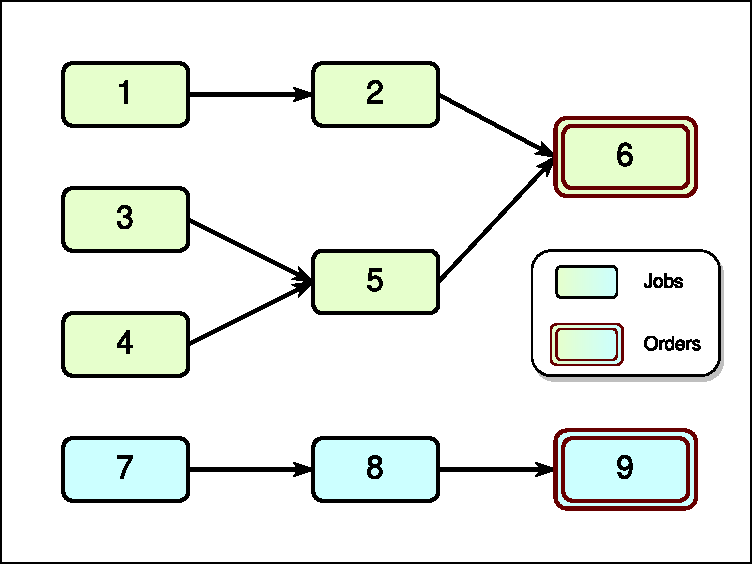
\includegraphics[width=0.6\textwidth]{img/Inforest.pdf}
    \caption{
        Example of a precedence graph.
        The inforest structure of the graph is demonstrated.
        Additionally, orders as the roots of the intrees are highlighted.}
    \label{fig:inforest}
\end{figure}

\begin{figure}[p]
    \centering
    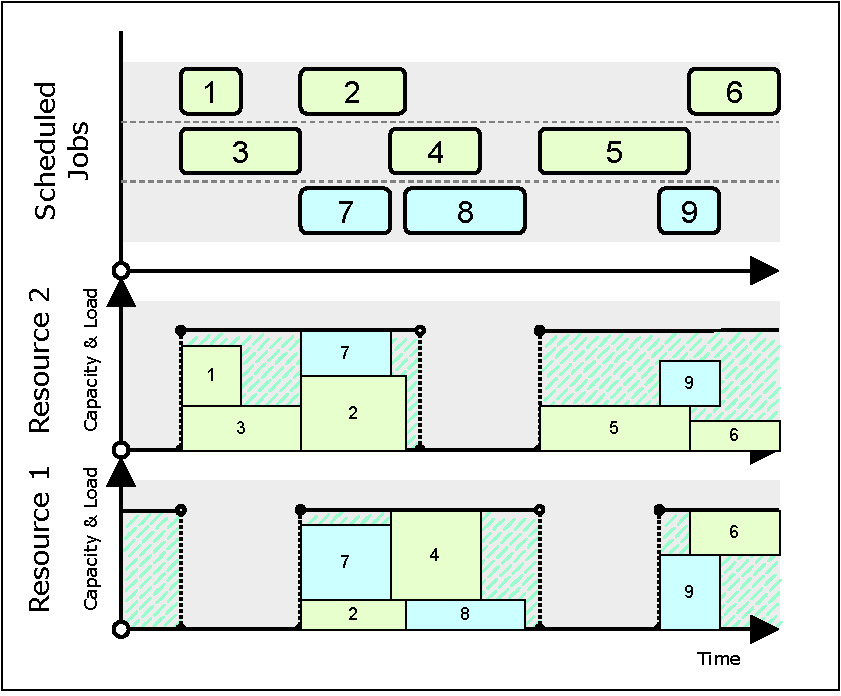
\includegraphics[width=0.999\textwidth]{img/Schedule.pdf}
    \caption{
        Example of a scheduled \ac{rcpsp} with time-variable resource capacities.
        The jobs with corresponding precedences from \cref{fig:inforest} are scheduled
        on two machines with partially overlapping working shifts.
        Job durations and capacity consumptions were chosen to illustrate the variability
        in resource utilization.
    }
    \label{fig:schedule}
\end{figure}

Each job $j \in \Jobs$ has a \emph{duration} $\duration{j}$,
describing the amount of time needed to process the job $j$.
\emph{Preemption} of jobs is not allowed in any form
--- the execution of a job cannot be interrupted after its start,
not even at the ends of working shifts (see variable resource capacities below).
Each job $j$ also has a \emph{due date}~$\deadline{j}$,
stating a time horizon in which the job should be completed;
otherwise, it is considered \emph{tardy}.
Subsequently, each job $j$ also has a \emph{tardiness weight} $\tardinessweight{j}$
which defines a penalty accumulated for each unit of time the job is tardy.

Execution order of jobs is constrained with \emph{precedence constraints} $\Precedences$.
A precedence constraint between jobs $i$ and $j$,
denoted as $\precedence{i}{j}$ or $(i, j) \in \Precedences$,
states that the processing of job $j$ can start only after the processing of job $i$ was completed.

Interpreting jobs $\Jobs$ as vertices and precedences $\Precedences$ as edges between the jobs,
we define the \emph{precedence graph} $G = (\Jobs, \Precedences)$.
We assume the precedence graph to be an \emph{inforest}, in other words,
the precedences constrain the execution order of jobs in such a way that the resulting precedence graph
is always an inforest.
An~inforest is a directed acyclic graph where each vertex has at most one successor.
A connected subgraph of an inforest is an \emph{intree}.
See \cref{fig:inforest} for a precedence graph example.

Jobs are executed on \emph{resources} $\Resources$ --- machines with time-variant renewable \emph{capacities}.
The capacity of a resource $k$ during a time period $t \in \intinterval{1}{\horizon}$ is denoted as $\capacity{k}{t}$.
During their execution, jobs consume the capacities of resources.
For a job $j$, the per-period consumption of a resource $k$ is denoted as $\consumption{j}{k}$.
This describes how much of the resource's capacity is consumed each period during the job's execution.
Capacities are renewable, meaning that each time period the specified amount of capacity is available,
regardless of prior capacity consumptions.
The resource capacity functions $\capacity{k}{t}$ are assumed periodic with the same period of 24.
Moreover, the resource capacity function of the resource $k$ only takes the values
$0$ and $\shiftcapacity{k} \negmedspace>\! 0$.
This assumption, however, is only for the initial problem instance
--- resource capacity functions of modified instances, as described in \cref{sec:problem-statement/relaxed-schedule},
can be non-periodical and take arbitrary non-negative integer values.

The set of \emph{orders} $\Orders = \{ j \in \Jobs \mid \nexists i : \precedence{j}{i} \}$
is the set of roots of the precedence intrees,
i.e. the set of all jobs for which no precedence successor exists.
A job $j \in \Orders$ is called an \emph{order}.

We make a simple observation; due to the intree-structure,
each (weakly) connected component in the precedence graph contains exactly one order.
From this, we can say that each job is either an order
or is associated with a unique order within the same intree component.
This is demonstrated in \cref{fig:inforest}.

Having introduced orders, we can now specify the ranges of job deadlines and tardiness weights
based on whether a job belongs to the orders set $\Orders$:

$$
\deadline{j} = \begin{cases}
    a \in \Nzero  &\dots\;   \text{if $j \in \Orders$} \\
    +\infty       &\dots\;   \text{otherwise}
\end{cases}
\qquad
\tardinessweight{j} = \begin{cases}
    a \geq 0  &\dots\;   \text{if $j     \in \Orders$} \\
    0         &\dots\;   \text{otherwise}
\end{cases}
$$

% ~~~~~~~~~~~~~~~~~~~~~~~~~~~~~~~~~~~~~~~~~~~~~~~~~~~~~~~~~~~~~~~~~~~~~~~~~~~~~~~~~~~~~~~~~~~~~~~~~~~~~~~~~~~
\section{Constraint programming model} \label{sec:problem-statement/constraint-programming-model}

We formulate the above problem using a constraint programming model.
This provides us with a well-functioning framework
and allows us to use existing solvers for finding optimal solutions.
The model can be stated as:

\begin{align}
    \text{given}      && \multicolumn{4}{l}{$\Jobs = (1, \dots, n) ,\;%
                                             \Resources = (1, \dots, m) ,\;%
                                             \Precedences ,\;%
                                             $} \nonumber \\
                      && \multicolumn{4}{l}{$\duration{1}, \dots, \duration{n} \in \Nzero ,\;%
                                             \deadline{1}, \dots, \deadline{n} \in \intinterval{1}{\horizon} ,\;%
                                             \tardinessweight{1}, \dots, \tardinessweight{n} \in \Nzero ,\;%
                                             $} \nonumber \\
                      && \multicolumn{4}{l}{$\consumption{1}{1}, \dots, \consumption{n}{m} \in \Nzero ,\;%
                                             \capacityf{1}, \dots, \capacityf{m} : \intinterval{1}{\horizon} \to \Nzero %
                                             $} \nonumber \\
    \text{find}       && \multicolumn{4}{l}{$\Schedule = (\jobstart{1}, \dots, \jobstart{n}) \in \N^n$} \nonumber \\
    \text{minimizing} && \sum_{j \in \Jobs} \tardinessweight{j} \tardiness{j}
                      &
                      &&
                      \label{csp:objective} \\
    \text{subject to} && \jobend{i}
                      & \leq \jobstart{j}
                      && \forall \precedence{i}{j} \in \Precedences
                      \label{csp:precedences} \\
                      && \sum_{j \in \Jobs} \modelConsumption{j}{k}{t}
                      & \leq \capacity{k}{t}
                      && \forall t \in \intinterval{1}{\horizon} \; \forall k \in \Resources
                      \label{csp:capacities} \\
    \text{where}      && \multicolumn{4}{l}{$\Completions = (\jobstart{1} + \duration{1}, \dots, \jobstart{n} + \duration{n}) ,\;%
                                             \tardiness{j} = \max(0, \jobend{j} - \deadline{j}) ,\;%
                                             $} \nonumber \\
                      && \multicolumn{4}{l}{$\modelConsumption{j}{k}{t} \defeq \begin{cases}
                                                 \consumption{j}{k} & \text{if $\jobstart{j} \leq t < \jobend{j}$} \\
                                                 0                  & \text{otherwise}
                                                 \end{cases}
                                             $} \nonumber
\end{align}

Inequalities \eqref{csp:precedences} formulate the precedence constraints --- start and finish times of jobs
are according to all the precedences.
Inequalities \eqref{csp:capacities} formulate the resource capacity constraints --- in every time period
the combined consumption of jobs scheduled during the period cannot exceed any of the resource's capacities.
Expression \eqref{csp:objective} is the optimization minimization objective --- the weighted tardiness of jobs.

We assume we have a solver capable of solving \eqref{csp:objective}--\eqref{csp:capacities} in reasonable time
through the use of constraint programming.

In the following sections, we will consider the stated constraints as potential bottlenecks
and how to relax specific constraints identified as bottlenecks.

% ~~~~~~~~~~~~~~~~~~~~~~~~~~~~~~~~~~~~~~~~~~~~~~~~~~~~~~~~~~~~~~~~~~~~~~~~~~~~~~~~~~~~~~~~~~~~~~~~~~~~~~~~~~~
\section{Bottlenecks} \label{sec:problem-statement/bottlenecks}

% -----------------------------------------------------------------------------------------------------------
\subsection{Definition} \label{subsec:problem-statement/bottlenecks/definition}

Our goal will be to find bottlenecks in the problem, specifically in the obtained schedule
--- the solution to the constraint programming model defined in \cref{sec:problem-statement/constraint-programming-model}.
First, we state a general definition of an execution-level bottleneck:

\begin{defn}[\acf{ebm} \citep{Wang2016}] \label{def:bottleneck}
    \emph{\ac{ebm}} is a machine that dominates the scheduling performance in the strongest manner
    at the execution level of production systems.
\end{defn}

The execution level of a production system stated here refers to finding bottlenecks
specific to the given problem instance and the obtained solution to that instance.
This is consistent with our goal of finding bottlenecks in the particular problem instances and their solutions,
and improving the system performance only with respect to the currently presented problem.
In contrast, we will not be interested in bottlenecks of the whole system
nor in generally improving the performance of the system regardless of the problem instance.
Having made the distinction, we will now discuss our interpretation of the definition suited to our problem.

Instead of identifying just a single machine as a bottleneck
or listing all the machines in the order of their scheduling impact,
we will focus on identifying specific time periods on specific machines as schedule bottlenecks.
This allows us to relax only the specific constraints related to the identified time periods,
resulting in localized modifications with minimal costs.

% -----------------------------------------------------------------------------------------------------------
\subsection{Constraints relaxation} \label{subsec:problem-statement/bottlenecks/constraints-relaxation}

When deciding which constraints to relax,
we have two constraints to consider: precedence constraints \eqref{csp:precedences}
and resource capacity constraints \eqref{csp:capacities}.
We will discuss individual segments that form the constraints,
considering their possible relaxation.

\begin{enumerate}[label=(\roman*)]
    \item \emph{Job precedences}
    Job precedence constraints are inherent to the problem ---
    --- jobs cannot start until all their predecessors have finished executing.
    We cannot remove individual precedences as a relaxation,
    as precedences model the technological requirements of the production system.
    We could imagine that scheduling jobs might require preparations,
    which do not necessarily require the presence of the product about to be processed.
    Those preparations could therefore be allowed to start even before the predecessor jobs finish executing,
    which would introduce slack in the constraints%
    \footnote{
    Scheduling with so-called \emph{setup times} is a broadly studied subject in the literature.
    See the survey of \citet{Hartmann2010} where the extension of setup times is described
    and various examples of approaches to the problem are given.
    }.
    However, we can assume that those preparations are completed before the start,
    or we can assume no preparation time at all.

    \item \emph{Cumulative consumption}
    The cumulative consumption is dependent on the constructed schedule and the given problem instance.
    Each job contributes to the cumulative consumption during the time periods it is scheduled.
    As part of the problem definition, we cannot omit this contribution,
    nor can it be shortened, as job durations $\duration{j}$ are fixed.
    Equally, job resource consumptions $\consumption{j}{k}$ influence the cumulative value,
    but again, due to the nature of our problem,
    we cannot modify resource consumptions as those are inherent to the problem
    and the corresponding real-life execution and operation requirements.

    \item \emph{Resource capacities}
    Available capacities of resources can be modified with reasonable correspondence
    to modifications of the real-life problem.
    More specifically, the capacity of a resource during a time period can be increased or decreased.
    Increasing the capacity of a resource during specific time periods could correspond to increasing
    the number of workers operating the resource machine,
    assuming that increasing the number of operating workers increases the total processing capacity.
    While sole reduction of capacities would not relax the constraints,
    decreasing the capacity of one resource by a specific amount
    while increasing the capacity of another resource
    by the same amount could tighten the constraints on the former resource
    but relax the constraints on the latter.
    This decreasing of the capacity of one resource
    while increasing the capacity of another by the same amount
    could correspond to migrating workers between the resource machines,
    assuming that migrations of operating workers are possible.
\end{enumerate}

We can conclude that the precedence constraints \eqref{csp:precedences} cannot be relaxed.
On the other hand, the resource capacity constraints \eqref{csp:capacities}
can be relaxed by modifying the capacities of resources.
As discussed,
these modifications can be achieved through capacity additions or migrations,
both of which have corresponding realizations in real-world production systems.

% -----------------------------------------------------------------------------------------------------------
\subsection{Resource capacity modifications} \label{subsec:problem-statement/bottlenecks/resource-capacity-modifications}

We will consider \emph{capacity additions} and \emph{capacity migrations} as the possible relaxations
of scheduling constraints, namely of the constraints \eqref{csp:capacities}.
Additions are executed by increasing the capacity of a selected resource
by a specified amount over a specified time interval.
Migrations are executed by decreasing the capacity of a selected source resource
by a specified amount over a specified time interval
and increasing the capacity of a selected target resource
by the specified amount over the same time interval.
An illustrative example of a capacity addition and a capacity migration is shown in \cref{fig:CapacityChanges}.

We consider migrations only between resources, limited to the same time interval.
We do not allow migrations in time ---
reducing the capacity of the source resource during a time interval
and then increasing the capacity of a target resource during a different interval.
Such migrations could correspond to migrating resource materials between resources.
In such cases, the change in time would correspond to the migrated material
being processed at a different time on a different machine.
However, we consider production systems with workers and machine operators as main resource capacities.
Considering this, migrating capacities in time would not have practical realizations,
as the workers migrated from one resource during one time period
would likely still be assigned to that resource during a different time period.

\begin{figure}
    \centering
    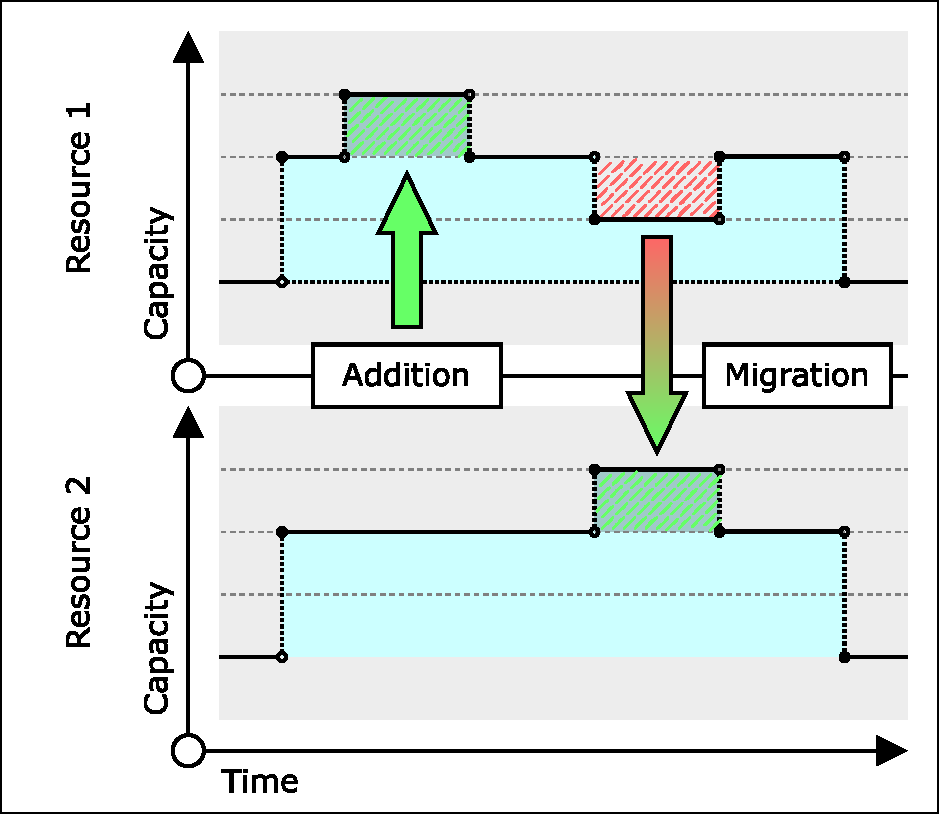
\includegraphics[width=0.7\textwidth]{img/Capacities-Changes.pdf}
    \caption{Diagram of possible capacity changes}
    \label{fig:CapacityChanges}
\end{figure}

We associate a capacity addition with the 4-tuple $\addition{k}{s}{e}{c}$, where
$k$ is the resource whose capacity is increased,
$s$ and $e$ form the time interval $\intinterval{s}{e-1}$ over which the addition is executed, and
$c$ is the added capacity.
Analogously, we associate a capacity migration
with the 5-tuple $\migration{k_{\text{from}}}{k_{\text{to}}}{s}{e}{c}$, where
$k_{\text{from}}$ is the source resource whose capacity is lowered,
$k_{\text{to}}$ is the target resource whose capacity is increased,
$s$ and $e$ form the time interval $\intinterval{s}{e-1}$ over which the migration is executed, and
$c$ is the migrated capacity.
For a modified instance $\Instance^*$, the sets of all migrations and additions are denoted as
$\Migrations^{\Instance^*}$ and $\Additions^{\Instance^*}$, respectively.

In a real-world production system,
migrating capacities is generally more cost-effective than adding new capacities.
For example, reassigning workers from an underutilized machine to a bottleneck machine
is typically less expensive than extending workers' shifts into overtime
or planning an entirely new and irregular shift.
Therefore, capacity migrations are usually preferred.
However, if the required capacity changes cannot be achieved through capacity migrations,
capacity additions can be utilized.

% ~~~~~~~~~~~~~~~~~~~~~~~~~~~~~~~~~~~~~~~~~~~~~~~~~~~~~~~~~~~~~~~~~~~~~~~~~~~~~~~~~~~~~~~~~~~~~~~~~~~~~~~~~~~
\section{Relaxed schedule} \label{sec:problem-statement/relaxed-schedule}

In the rest of this chapter, we define a general procedure for solving the presented problem,
identifying bottlenecks and relaxing corresponding constraints by modifying the initial problem,
solving the modified problem,
and evaluating whether the modified solution reached a desired improvement.
More precisely:

\begin{enumerate}
    \item Suppose we obtained an optimal solution $\Schedule$ to the problem instance $\Instance$.

    \item We select the target order $\targetOrder \in \Orders$ for which we want to improve the tardiness.
        We consider improvement to be any non-zero decrease in the objective function with respect to the
        selected order $\targetOrder$ and its tardiness $\tardiness{\targetOrder}$.

    \item We identify bottlenecks in the solution $\Schedule$ of the instance $\Instance$.

    \item Based on the identified bottlenecks, corresponding constraints are relaxed via
        capacity additions and capacity migrations.
        Those capacity changes are captured by modified resource capacity functions
        $\capacityf{1}^*, \ldots, \capacityf{m}^*$
        corresponding to a modified problem instance $\Instance^*$.

    \item We obtain a solution $\Schedule^*$ to the modified problem instance $\Instance^*$.

    \item Finally, any desired evaluations can be made on the modified solution $\Schedule^*$,
        alongside comparisons to the original solution $\Schedule$.
\end{enumerate}

\chapter{Related works} \label{chap:related-works}

% ~~~~~~~~~~~~~~~~~~~~~~~~~~~~~~~~~~~~~~~~~~~~~~~~~~~~~~~~~~~~~~~~~~~~~~~~~~~~~~~~~~~~~~~~~~~~~~~~~~~~~~~~~~~
\section{\acs{rcpsp} scheduling} \label{sec:related-works/scheduling-the-rcpsp}

To model our studied problem we chose the \Problem{} version of the \ac{rcpsp}.
The standard \ac{rcpsp} is proven to be NP-hard \citep{Blazewicz1983}.
A comprehensive overview of complexity results was done by \citet{Ganian2021}.

% -----------------------------------------------------------------------------------------------------------
\subsection{Time-variable resource capacity constraints} \label{subsec:related-works/scheduling-the-rcpsp/time-variable-resource-capacity-constraints}

Under the general $PSm$ (Project Scheduling) characteristic we allow arbitrary resource capacity functions.
However, as stated in \cref{sec:problem-statement/scheduling,sec:problem-statement/bottlenecks,sec:problem-statement/relaxed-schedule},
the resource functions are mostly periodical with only a few local modifications.

\citet{Hartmann2010} and \citet{Hartmann2022} surveyed the variants of the \ac{rcpsp} studied in the literature
and alongside other variants also discussed time-variable resource capacity constraints.
As in our modeled real-world problem,
the surveyed literature used the time-varying capacities to model worker shifts,
resource machine maintenance, or other manufacturing processes resulting in variable availabilities.

Time-variable resource availabilities are often studied with allowed preemption.
Recall from \cref{sec:problem-statement/scheduling} that when job preemption is allowed,
execution of a job can be interrupted and resumed at a later period.
Usually, only a specific form of preemption is allowed ---
interrupting the execution of a job at the end of a working shift
and resuming it at the start of the following working shift.
Preemption in this context can be a reasonable assumption as it can,
in some manufacturing systems, correspond to a simple interruption in executed work.
On the other hand, job preemption, even in the specific form mentioned,
might not be available due to technical reasons.

To state a few examples of scheduling under time-variable resource capacity constraints,
see the work of \citet{Klein2000} or \citet{Nonobe2002}.
For an example of calendar-based availability scheduling with job preemption, see the work of \citet{Franck2001}.

% -----------------------------------------------------------------------------------------------------------
\subsection{Solution approaches} \label{subsec:related-works/scheduling-the-rcpsp/solution-approaches}

Solving the \ac{rcpsp} is done using exact methods, heuristics, or metaheuristics.
Exact solution methods aim to solve scheduling problems systematically.
They guarantee to find the optimal solution by exhaustively exploring all possible solutions
within a problem's feasible solution space.
However, this exhaustive search can become computationally expensive
and impractical for large-scale or complex problem instances.
The most prominent exact approach is the branch-and-bound method,
used in many variations and with problem-specific heuristics.
First branch-and-bound solution method was proposed by \citet{Demeulemeester1992},
another example is the work of \citet{Vanhoucke2001}.
An approach using a modified constraint programming and SAT solver
with generalized precedence relations can be found in the work of \citet{Schnell2015}.

In contrast, heuristics aim to quickly find good solutions but do not guarantee optimality.
Heuristic approaches are simple, easy to implement, and computationally inexpensive compared to exact methods.
Heuristics use priority scheduling rules, schedule-generating schemes, and approximations,
but also relaxations of exact methods, such as truncated branch-and-bound or relaxed integer programming.
Simple heuristics were popular as alternatives to exact methods.
See the survey of \citet{Kolisch1999} for an extensive survey of heuristic approaches used at the time.

Metaheuristics are higher-level problem-solving frameworks that search for good solutions
in the solution space using a combination of exploration and exploitation strategies.
Like simple heuristics, metaheuristics do not guarantee finding the optimal solution
but offer a trade-off of computational performance.
They are often more complex than simple heuristics and, as a result computationally more expensive,
but they can handle larger and more complex problem instances.
Metaheuristics include genetic algorithms, simulated annealing, tabu search, and particle swarm optimization.
A recent survey on metaheuristics by \citet{Pellerin2020} compares a wide range of metaheuristics
on PSPLIB instances.

We chose an exact solution approach by utilizing a constraint programming solver.
Our problem contains many constraints, most of which model time-variable capacities of resources.
We frequently modify those constraints and, therefore, need to make adjustments to the model.
Constraint programming models and solvers are ideal for such use cases.
The constraints can be expressed in a declarative way without having to handle specifics.
This makes the process of adjusting the declared constraints and obtaining modified models straightforward.
In comparison, modeling these problems for heuristics or metaheuristics requires significantly more effort,
and adjusting the modeled constraints might prove even more difficult.

% ~~~~~~~~~~~~~~~~~~~~~~~~~~~~~~~~~~~~~~~~~~~~~~~~~~~~~~~~~~~~~~~~~~~~~~~~~~~~~~~~~~~~~~~~~~~~~~~~~~~~~~~~~~~
\section{Bottlenecks in scheduling} \label{sec:related-works/bottlenecks-in-scheduling}

Bottlenecks are broadly studied in the scheduling literature.
The notion of a bottleneck is recognized to have an important role in scheduling when system performance is considered.

% -----------------------------------------------------------------------------------------------------------
\subsection{Various definitions} \label{subsec:related-works/bottlenecks-in-scheduling/various-definitions}

In \Cref{def:bottleneck} we defined the \acf{ebm}.
We chose this definition as it best corresponds to our studied problem.
Namely, it emphasizes the execution phase of production within which the bottleneck is considered
and doesn't specify any particular metric or measure of the bottleneck's impact on the system.

\citet{Betterton2012} surveyed the literature on scheduling bottlenecks and found
at least 11 different definitions of the term \emph{bottleneck resource}.
The first attempts at defining the term were very specific in the way the bottleneck resource is identified.
Usually, the definition corresponded closely with the identification method proposed in the same work.
See for example the work of \citet{Lawrence1994}, \citet{Kuo1996}, or \citet{Roser2001}.
Throughout the years, however, the aim shifted towards defining a bottleneck as generally as possible
to cover as many specific interpretations of the term
but to also best capture the important nature of a bottleneck resource in production systems.
For attempts at this approach see the work of \citet{Chiang2001} or \citet{Biller2010}.

Based on the definitions presented up to that point,
\citet{Betterton2012} stated the following definition.

\begin{defn}[Bottleneck resource \citep{Betterton2012}] \label{def:bottleneck-general}
    The \emph{bottleneck} is the resource that affects the performance of a system in the strongest manner, that is,
    the resource that, for a given differential increment of change, has the largest influence on system performance.
\end{defn}

This definition provides a neat generalization of the term \emph{bottleneck resource}.
It also provides insight that focusing on such resources and making small adjustments
can significantly influence the system's performance.
Note, that the definition does not specify the influence of mentioned adjustments has to be beneficial towards the performance.
Correctly identifying the bottleneck resource, but incorrectly adjusting the related settings can impact the performance negatively.

% -----------------------------------------------------------------------------------------------------------
\subsection{Bottleneck classification} \label{subsec:related-works/bottlenecks-in-scheduling/bottleneck-classification}

Bottlenecks can be identified at different stages of production.
We use the bottleneck classification proposed by \citet{Wang2016}.
This classification distinguishes between structural, planning, and execution bottlenecks
based on the time frame at which the bottlenecks are identified.

\emph{Structural bottleneck machines} frequently affect the performance of the production system,
regardless of the specific problem setting.
Such machines are usually identifiable by human operators,
as their high impact on performance can be observed across different problem settings and schedules.
In contrast to their identifiability by humans, structural bottlenecks might not be easily solvable or relaxed.
It may be caused by a hard limitation of the system,
for example, an inefficient production line layout or
machines running at full capacity without the possibility of increasing the capacity.

Structural bottlenecks can be identified with the use of historical production data.
Modern production systems collect large volumes of data concerning the production,
performance of individual components, utilization of resources, etc.
This data is then processed by techniques from data science or machine learning
to capture various patterns in production, anomalies, or correlations among the data
indicating a potential bottleneck.
Such techniques can better react and adapt to dynamic changes in the production system,
given that enough data regarding similar dynamic changes has been collected.
A recent survey by \citet{Subramaniyan2021} provides an overview of data-driven bottleneck identification methods.
To state a few examples, see the work of \citet{Subramaniyan2016}, \citet{Roh2018} or \citet{Li2009}.

When historical data is not available,
a simulation of the system might provide a sufficient approximation of the real production.
Such an approach was studied by \citet{Roser2001} where the study focused on a serial production line
and the bottleneck machine was identified through the average active duration on machines.
\citet{Zhang2008a} and \citet{Zhang2012} first model an alternative relaxed optimization model for the system,
identify the bottleneck machines during the scheduling of this model,
and then schedule the original problem with a designed genetic algorithm,
which utilizes the obtained bottleneck information by allocating more resources to the identified machines.

\emph{Planning bottleneck machines} are considered during the construction of a schedule.
Identifying such machines during the scheduling process can help guide the scheduling procedure
--- whether exact, heuristic, or metaheuristic.
The scheduling procedure can choose to allocate more resources to the identified bottleneck machine,
spend more time and computational resources on scheduling jobs on such machines, etc.
A notable example of such an approach is the shifting bottleneck procedure proposed by \citet{Adams1988}.
They construct the schedule by sequentially scheduling on singular machines,
each time choosing an unscheduled machine identified as the current bottleneck,
then locally reoptimizing the already scheduled machines.
In their study, \citet{Mnch2010} argue that the shifting bottleneck procedure in its various versions
remains a superior method for scheduling semiconductor wafer production systems.
They argue that this is due to several difficulties present in scheduling such systems,
challenges that the shifting bottleneck procedure can easily address.
In a Job-Shop scheduling problem,
\citet{Zhang2008b} identify bottleneck machines by their sensitivity to changes to their scheduling policies.
They incorporate this identification in a proposed genetic algorithm to guide its search for improved solutions.

\emph{Execution bottleneck machines} are the focus of study in this thesis.
These bottlenecks are considered in the constructed schedule for a given problem instance
and restrain us from achieving a better schedule in terms of the given optimization goal,
such as average throughput, schedule makespan, weighted tardiness, etc.
While identifying structural bottlenecks primarily aims to enhance the overall system performance,
identifying execution bottlenecks aims to improve performance for specific problem instances.
It's worth noting that for a specific problem instance and its constructed schedule,
we may identify one machine as its execution bottleneck,
but for a different problem instance with different settings,
the execution bottleneck may vary.
Consequently, relaxing constraints related to an identified execution bottleneck
aims to enhance performance for the specific problem instance;
however, applying such relaxation to a different problem instance might not provide any improvement.

Limited studies have focused on this type of bottleneck.
\citet{Wang2016} proposed a multi-indicator approach for identifying execution bottlenecks.
Their study investigated how identified execution bottlenecks differ from identified planning bottlenecks.
Computational results demonstrate that, for many problems,
the identified planning bottlenecks differ from the execution bottlenecks identified in specific schedules for those problems.
This highlights the importance of distinguishing between planning bottlenecks and execution bottlenecks.

% -----------------------------------------------------------------------------------------------------------
\subsection{Identification indicators} \label{subsec:related-works/bottlenecks-in-scheduling/identification-indicators}

Various techniques are used for the identification of bottleneck machines.
Such techniques typically involve the usage of identification indicators,
either individually or in combination.
An identification indicator refers to a value computed for each machine,
allowing us to rank the machines and then select the bottleneck machine based on this rank.
We will state a few examples proposed in the literature:

\begin{itemize}
    \item \acf{mur} \citep{Lawrence1994}:
    $$
    \indMUR{k} = \frac{\sum_{j \in \JobsOnResource{k}} \duration{j}}%
                      {\max_{j \in \JobsOnResource{k}} \jobend{j}
                       - \min_{j \in \JobsOnResource{k}} \jobstart{j}}.
    $$

    \item \acf{ql} \citep{Lawrence1994}.
    In manufacturing systems consisting of machines with workload queues,
    this indicator considers the number of items in the machine's queue as the bottleneck measure.
    
    \item \acf{auad} \citep{Roser2001}:
    $$
    \indAUAD{k} = \frac{\sum_{i=1}^{A_k} a_{ki}}{A_k},
    $$
    where $a_{k1}, \dots, a_{kA_k}$ are the lengths of uninterrupted active durations of resource $k$,
    $A_k$ is the number of those individual durations.

    \item \acf{rs} \citep{Cooper1976}
        and \acf{rc} \citep{Patterson1976}:
        \begin{align*}
        \indRS{k} &= \frac{R_{k}}%
                          {\avg_{j \in \Jobs} \consumption{j}{k}}
                  = \frac{R_{k} \cdot n}%
                         {\sum_{j \in \Jobs} \consumption{j}{k}},
        \\[1em]
        \indRC{k} &= \frac{\avg_{j \in \JobsOnResource{k}} \consumption{j}{k}}%
                          {R_{k}}
                   = \frac{\sum_{j \in \JobsOnResource{k}} \consumption{j}{k}}%
                          {R_{k} \cdot |\JobsOnResource{k}|},
        \end{align*}
        where $R_{k}$ is the per-period capacity of a resource $k$ ---
        these indicators do not account for variable resource capacities.
        Those indicators are usually considered when describing problem instances,
        specifically, the properties of resources.
        However, \citet{Luo2023} chose them as bottleneck identifiers
        and compared their effectiveness when used to guide a genetic programming algorithm.
\end{itemize}

In the formulae for $\indMUR{k}$ and $\indRC{k}$,
$\JobsOnResource{k} \defeq \{j \in \Jobs : \consumption{j}{k} > 0\}$
is the set of jobs with nonzero consumption of the resource $k$,
i.e. the jobs which are executed on the resource $k$.

Identification indicators have the advantage of being simple,
making their implementation straightforward and their computation efficient.
However, more complex identification methods may provide better insights
into the bottleneck identification process.
Nevertheless, these methods are usually tailored specifically to the problem being studied,
require specific settings and assumptions,
or their implementation can be too complicated for practical use.

% -----------------------------------------------------------------------------------------------------------
\subsection{Bottlenecks in the \acs{rcpsp}} \label{subsec:related-works/bottlenecks-in-scheduling/bottlenecks-in-the-rcpsp}

To the best of our knowledge, only little research focuses on identifying bottlenecks in the \ac{rcpsp}.
The closest research is on bottlenecks in the Job-Shop problem,
i.e. scheduling on unit-capacity resources.

\citet{Luo2023} studied how identifying bottleneck machines can guide the scheduling
process of a genetic algorithm.
\citet{Arkhipov2017} conducted a case study on a large-scale resource-constrained scheduling problem
with over 3 thousand operations and over 50 machines.
To address this problem, they proposed a heuristic approach for estimating project makespan
and resource load profiles.
Those estimations are in turn used to identify bottleneck resources for the problem.
However, the identified bottleneck resources were not addressed further.

Concerning bottleneck identification indicators discussed above,
we were unable to find any for the \ac{rcpsp} with time-variable resource capacities.
Moreover, we were unable to find any identification identifiers for the standard \ac{rcpsp}
which would account for time-variable consumption profiles in a schedule.
Although the indicators mentioned in \cref{subsec:related-works/bottlenecks-in-scheduling/identification-indicators}
can in theory be used in the \ac{rcpsp},
they were originally designed for the Job-Shop problem.
Identification indicators in the \ac{rcpsp} could incorporate information about
variable resource loads and even
variable capacity functions in the time-variant capacities extension.
However, the indicators designed for the Job-Shop problem do not consider
this additional dimension of information.
We address this further in \cref{sec:solution-apporach/baseline-solution}.

% -----------------------------------------------------------------------------------------------------------
\subsection{Relaxing the identified bottlenecks} \label{subsec:related-works/bottlenecks-in-scheduling/relaxing-bottlenecks}

In their study, \citet{Zhang2012} addressed the Job-Shop problem by relaxing its capacity constraints
and then solving the modified relaxed problem to identify bottlenecks based on the solution.
The obtained information was used to guide a proposed simulated annealing
algorithm to find a solution to the original problem.
Thus, the relaxation served only as an intermediate step toward obtaining a solution,
rather than being the desired result.

\citet{Lawrence1994} studied how identified bottlenecks shift between machines
in response to introducing relaxations to the original problem.
They employed a proposed "bottleneck chasing" policy for relaxing short-run bottlenecks,
wherein the capacity of the identified bottleneck resource is increased,
e.g., by extending its working shifts, or assigning additional employees.
Then, the bottleneck identification process is run again to examine
whether the bottlenecks shift to a different resource.
The sensitivity of bottleneck shifting to the introduced relaxations was also studied.
The authors observed that while the chasing policy is effective at relaxing local bottlenecks,
it also increases the \enquote{bottleneck shiftiness,}
resulting in a more change-sensitive system.
They also studied the shiftiness of long-run bottleneck resources having the highest utilization over time.
Their results showed that increasing the capacity of bottleneck resources
to address long-run bottlenecks also increases the bottleneck shiftiness,
but this shiftiness can be reduced by simultaneously increasing the capacity of non-bottleneck
resources.

\section{Contribution} \label{sec:related-works/contribution}

As discussed in \cref{subsec:related-works/bottlenecks-in-scheduling/identification-indicators,subsec:related-works/bottlenecks-in-scheduling/bottlenecks-in-the-rcpsp},
the scheduling literature primarily focuses on bottlenecks in the Job-Shop problem.
We aim to extend the standard Job-Shop approaches to the \ac{rcpsp}.
Our second goal is to design an approach for identifying bottlenecks in the \ac{rcpsp}
extended with time-variant resource capacities
with the focus on relaxing the identified bottlenecks to improve a proposed schedule.

\chapter{Solution approach} \label{chap:solution-apporach}

In this chapter,
we present two algorithms designed for identifying and relaxing bottlenecks in the \ac{rcpsp}.
Both algorithms aim to improve the tardiness of a selected order
by introducing relaxations to the capacity constraints in the problem instance
and finding a solution to the modified problem instance.

First, we propose an algorithm called \acf{iira}.
The \ac{iira} combines an adaptation of existing bottleneck identification approaches from the literature
with a new method for relaxing the capacity constraints.
The algorithm utilizes bottleneck identification indicators to find bottleneck resources,
selects periods with high improvement potential,
and increases the capacities of the bottleneck resources during the selected periods.

The second algorithm we propose is the \acf{ssira}.
The \ac{ssira} employs a novel approach to relaxing capacity constraints
based on finding improvement intervals in partially relaxed versions of the problem.
\ac{ssira} iteratively relaxes the capacity constraints in suffixes of an obtained schedule
and selects jobs that could start earlier following the relaxation.
The resource capacity constraints are then relaxed with respect to a small subset
of the selected jobs with improvement potential.

To help explain how the algorithms work,
we illustrate\footnote{
    The figures used to illustrate the specifics of the algorithms were created in Python
    using the plotting library Matplotlib. See online at \url{https://matplotlib.org/}.
}
key moments on the schedule given in \cref{fig:example/base}.
In the illustrated schedule, job 9 is scheduled past its due date and is considered tardy.
This job is the target order for improvements in the examples provided for the algorithms.

\begin{figure}
    \centering
    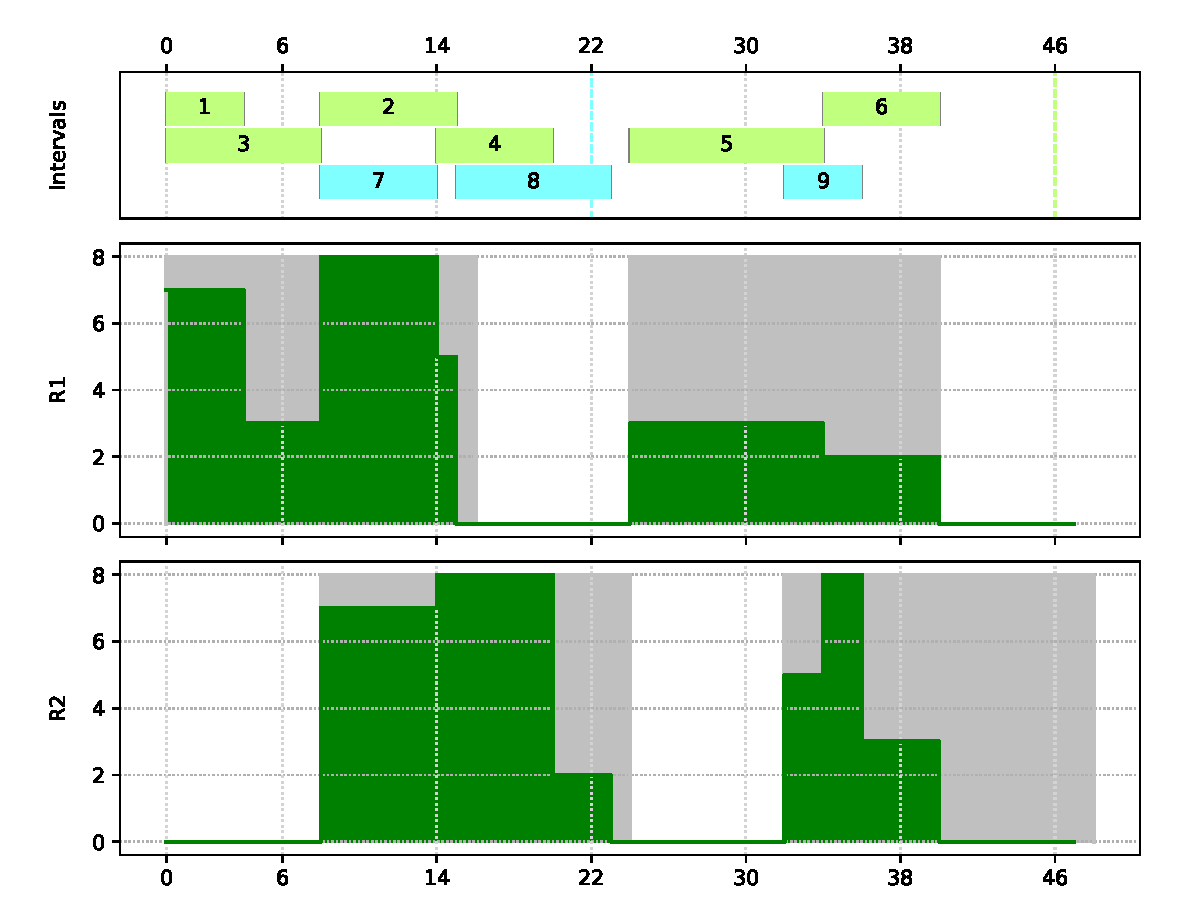
\includegraphics[width=\textwidth]{img/example_solution_base.pdf}
    \caption{
        Computed example schedule.
        Job 9 is considered tardy as it is scheduled past its due date (time period 22).
        }
    \label{fig:example/base}
\end{figure}

% ~~~~~~~~~~~~~~~~~~~~~~~~~~~~~~~~~~~~~~~~~~~~~~~~~~~~~~~~~~~~~~~~~~~~~~~~~~~~~~~~~~~~~~~~~~~~~~~~~~~~~~~~~~~
\section{Baseline solution} \label{sec:solution-apporach/baseline-solution}

In this section, we propose adaptations of existing bottleneck identification indicators from the literature.
Utilizing the adapted indicators, we propose the \ac{iira}
for relaxing capacity constraints of a given problem instance based on its solution.

% -----------------------------------------------------------------------------------------------------------
\subsection{Adapted identification indicators}

We adapt existing identification indicators to detect bottlenecks,
specifically the \acf{mur} and \acf{auad} indicators.
For precise definitions, see \cref{subsec:related-works/bottlenecks-in-scheduling/identification-indicators}.
        
The \ac{mur}, first utilized as a bottleneck identification indicator by \citet{Lawrence1994},
considers the ratio of executed work on a resource to the total time the resource was used.
In their study, \citet{Lawrence1994} demonstrate, that despite its simplicity,
the \ac{mur} indicator is effective at identifying long-run bottlenecks%
\footnote{
Long-run bottlenecks could be viewed as structural bottlenecks ---
see \cref{subsec:related-works/bottlenecks-in-scheduling/bottleneck-classification} for bottleneck classification.
}.


The \ac{auad}, initially proposed by \citet{Roser2001},
is more complex but remains a comprehensive indicator for identifying bottleneck resources.
For the specified resource, the sequence of all uninterrupted execution periods is computed
and the average length of those periods is considered the indicator value.
An uninterrupted period is a sequence of jobs scheduled consecutively with no idle times between them.
If there is an idle time period between two subsequent jobs,
they belong to different uninterrupted periods.

Both identification indicators consider the relationship between the total duration
of job executions on a resource and the duration for which the resource is idle.
In a Job-Shop scheduling problem,
this represents all the available information.
This concept remains applicable in the \ac{rcpsp}.
However, due to the variability of machine load over time in the \ac{rcpsp},
a binary \enquote{processing--idle} differentiation between machine states
does not provide a sufficient machine-load indication.
In the \ac{rcpsp}, we have additional information available.
By incorporating resource capacities and resource consumptions into the calculation,
we can achieve a more precise result that better corresponds to the actual machine load.
\cref{fig:MachineLoad} illustrates the difference in variability of the load between
a Job-Shop machine (\cref{fig:MachineLoad:JS})
and a \ac{rcpsp} machine (\cref{fig:MachineLoad:RCPSP}).

\begin{figure}[t]
    \centering
    
    \subfloat[Job-Shop scheduling problem]{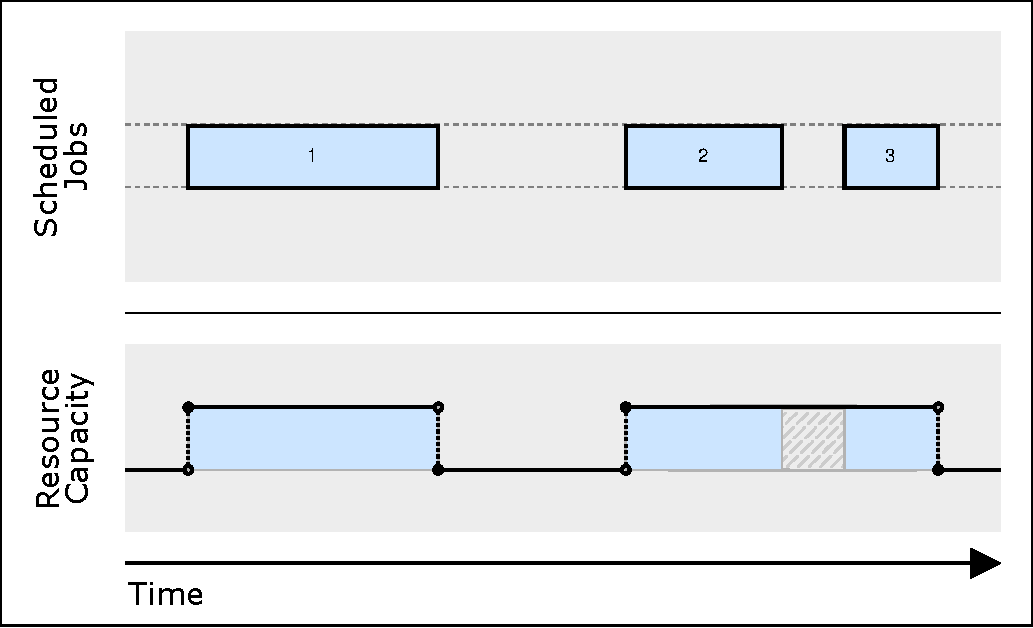
\includegraphics[width=0.7\textwidth]{img/Capacities-JobShop.pdf}\label{fig:MachineLoad:JS}}
    \\
    \subfloat[RCPSP]{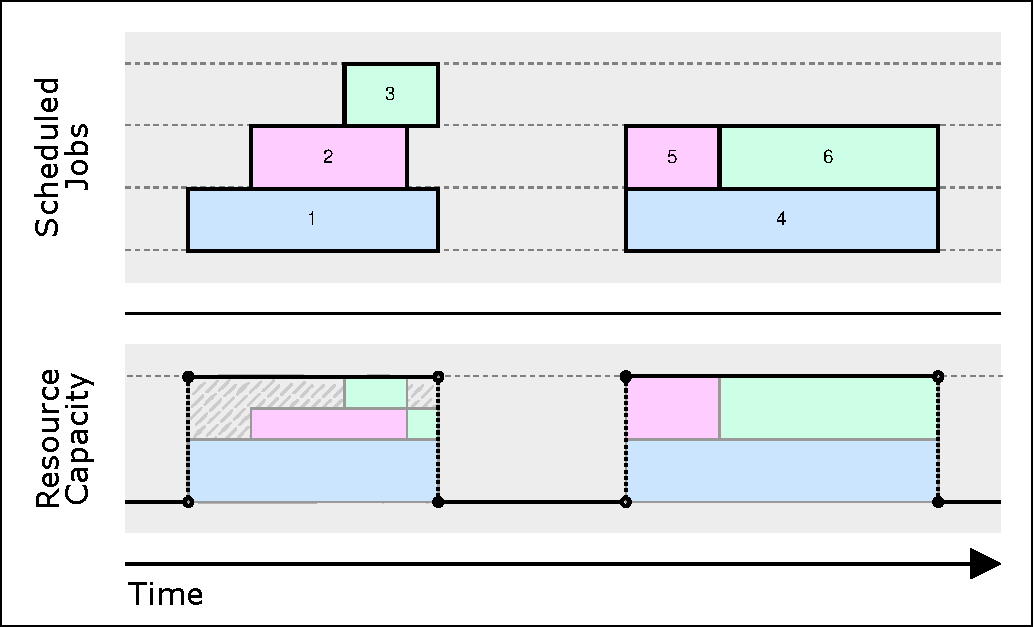
\includegraphics[width=0.7\textwidth]{img/Capacities-RCPSP.pdf}\label{fig:MachineLoad:RCPSP}}
    
    \caption{
        Examples of machine-load functions of the Job-Shop problem and the \ac{rcpsp} problem.
        The variability in the possible machine loads during job execution
        between the Job-Shop problem and the \ac{rcpsp}
        and the variability in machine loads during different periods in the \ac{rcpsp} are demonstrated.
        }
    \label{fig:MachineLoad}
\end{figure}

We propose \acf{mrur} as the adaptation of \ac{mur} and \acf{auau} as the adaptation of \ac{auad}.
For a resource $k$, the \ac{mrur} is defined as:
$$
\indMRUR{k} \defeq \frac{\sum_{j \in \Jobs} (\duration{j} \cdot \consumption{j}{k})}%
                        {\sum_{t=1}^{C_{\max}} \capacity{k}{t}},
$$
where $C_{\max} \defeq \max_{j \in \Jobs} \jobend{j}$%
\footnote{In the scheduling literature,
$C_{\max}$ is referred to as the \emph{makespan} of the project.
Minimizing project makespan is a common optimization goal in scheduling,
and it is a simpler alternative to the total weighted tardiness we use.}.
For a resource $k$, the \ac{auau} is defined as:
$$
\indAUAU{k} \defeq \frac{\sum_{i=1}^{A_k} \indPRU{k}{i}}%
                        {A_k},
$$
where the \acf{pru} of resource $k$ during the uninterrupted active period $i$
is defined as
$$
\indPRU{k}{i} \defeq \frac{\sum_{j \in \JobsOnResourceInPeriod{k}{i}}
                                \duration{j} \cdot \consumption{j}{k}}%
                          {\sum_{t=a_{ki}^{S}}^{a_{ki}^{E}} \capacity{k}{t} }.
$$
For a resource $k$,
$(a_{k1}^{S}, a_{k1}^{E}), \dots, (a_{kA_k}^{S}, a_{kA_k}^{E})$
is the the sequence of \emph{uninterrupted active periods},
where $a_{ki}^{S} \in \intinterval{1}{\horizon-1}$ denotes the start of the period $i$
and $a_{ki}^{E} \in \intinterval{a_{ki}^{S}+1}{\horizon}$ denotes the end of the period $i$.
Similar to the definition of \ac{auad} but with differences induced by non-unit capacities,
an uninterrupted active period is a maximal set (maximal in terms of inclusion)
of jobs scheduled consecutively or in parallel with no idle time
occurring on the considered resource during the period.
Two jobs are in the same uninterrupted active period, if and only if
the execution intervals of the jobs overlap
or the considered resource is not idle between the execution intervals of the jobs.
The sequence of uninterrupted active periods of a resource is the transitive closure of this relation
on jobs executed on the resource.
Here, as opposed to the \ac{auad},
we do not consider the duration of the periods,
but the individual jobs executed during each of the periods,
specifically their durations and consumptions of the evaluated resource.

In the formula for $\indPRU{k}{i}$,
$\JobsOnResourceInPeriod{k}{i} \defeq \{ j \in \JobsOnResource{k} : a_{ki}^{S} \leq \jobstart{j} \leq a_{ki}^{E} \}$
is the set of jobs executed on resource $k$ during the uninterrupted active period $i$.
Recall from \cref{subsec:related-works/bottlenecks-in-scheduling/identification-indicators} that
$\JobsOnResource{k} = \{ j \in \Jobs : \consumption{j}{k} > 0 \}$.

Having proposed bottleneck identification indicators for our \ac{rcpsp} variant,
we will formulate an algorithm utilizing those indicators in the following section.

% -----------------------------------------------------------------------------------------------------------
\subsection{Identification Indicator-based Relaxing Algorithm} \label{subsec:solution-approach/baseline-solution/iira}

In this section, we formulate the \acf{iira}.
\ac{iira} employs a specified bottleneck identification indicator to identify bottleneck resources.
It calculates the granular resource load function
and uses its convolution with a suitably chosen kernel function
to determine the improvement potential for granular periods.
Finally, it relaxes capacity constraints in granular periods with the greatest improvement potential.
Following this, a solution is obtained for the relaxed problem instance,
and the proposed capacity relaxations are reduced to only include those utilized by the new solution.
The \acf{iira} is given in \cref{alg:identification-indicator-relaxing-algorithm}.

\begin{algorithm}[t]
\caption{\acf{iira}}
\label{alg:identification-indicator-relaxing-algorithm}
\begin{algorithmic}[1]

\Params  Identification indicator $\algIndicator$, granularity $\algGranularity$, convolution mask $\algConvolution$,
\Paramsc iterations limit $\algMaxiter$, improvement periods limit $\algMaxperiods$,
\Paramsc capacity improvement $\algImprovement$
\Input  Solution $\Schedule$ to a problem instance $\Instance$

\State $PC \gets \lceil \horizon / \algGranularity \rceil$
       \Comment The number of granular periods
\State $\Instance^* \gets \Instance$, $\Schedule^* \gets \Schedule$
       \Comment Modified instance and its solution, initially
       \Statecr copies of the original instance and solution
\Repeat \label{alg:iira/repeat}
    \State Evaluate $\Schedule^*$ using $\algIndicator$, obtaining:
           $\algIndicator_k \;\forall k \in \Resources$ \label{alg:iira/evaluation}
    \State Identify bottleneck resource:
           $k^* \gets \argmax_k \algIndicator_k$ \label{alg:iira/identification}
    \State Compute granular resource load for $k^*$: \label{alg:iira/granular-load}
    \Statec{3} $\resourceLoad{k^*} \gets $ \Callref{GranularResourceLoad}%
                                                   {$k^*$, $\Instance^*$, $\Schedule^*$, $PC$}%
                                                   {alg:granular-resource-load}
    \State Compute improvement potential of periods: $\Psi \gets \resourceLoad{k^*} * \algConvolution$ \label{alg:iira/convolution}
    \State Find improvement periods: \label{alg:iira/periods}
    \Statec{3} $p_1, \dots, p_{\algMaxperiods} \gets$
            periods with the highest potential $\Psi(i)$
    \For {$i \in \{p_1, \dots, p_{\algMaxperiods}\}$}
        \State $\capacityf{k^*}^* \gets$ \Callref{IncreaseGranularPeriodCapacity}%
                                                 {$i$, $\capacityf{k^*}^*$, $\algGranularity$, $\algImprovement$}%
                                                 {alg:increase-granular-period-capacity} \label{alg:iira/capacity-increase}
    \EndFor
    \State Find solution $\Schedule^*$ to the modified instance $\Instance^*$ \label{alg:iira/modified-solution}
    \State $\capacityf{1}^*, \dots, \capacityf{m}^* \gets$ \Callref{ReduceCapacityChanges}%
                                                                   {$\Instance^*$, $\Schedule^*$, $\capacityf{1},$ \dots, $\capacityf{m}$}%
                                                                   {alg:reduce-capacity-changes} \label{alg:iira/reduction}
    \State $\Additions^{\Instance^*}, \Migrations^{\Instance^*} \gets $
           \Callref{FindAdditionsAndMigrations}%
                   {$\Instance^*$, $\Schedule^*$}%
                   {alg:find-additions-and-migrations} \label{alg:iira/additions-migrations}
\ForIter{$\algMaxiter$} \label{alg:iira/for-iters}

\Output  Modified instance $\Instance^*$ and its solution $\Schedule^*$,
\Outputc additions $\Additions^{\Instance^*}$, migrations $\Migrations^{\Instance^*}$
\Statex
\Note In the call to \Call{ReduceCapacityChanges}{} (statement 12),
      $\capacityf{k^*}$ from the~original instance is given as the original capacity function of the resource $k^*$.

\end{algorithmic}
\end{algorithm}

The algorithm consists of a main loop (lines~\ref{alg:iira/repeat}--\ref{alg:iira/for-iters}),
the input of which is a problem instance and its solution,
the output of which is a modified problem instance and its solution.
We describe the individual steps performed by the algorithm in the following outline.

\begin{figure}[p]
    \centering
    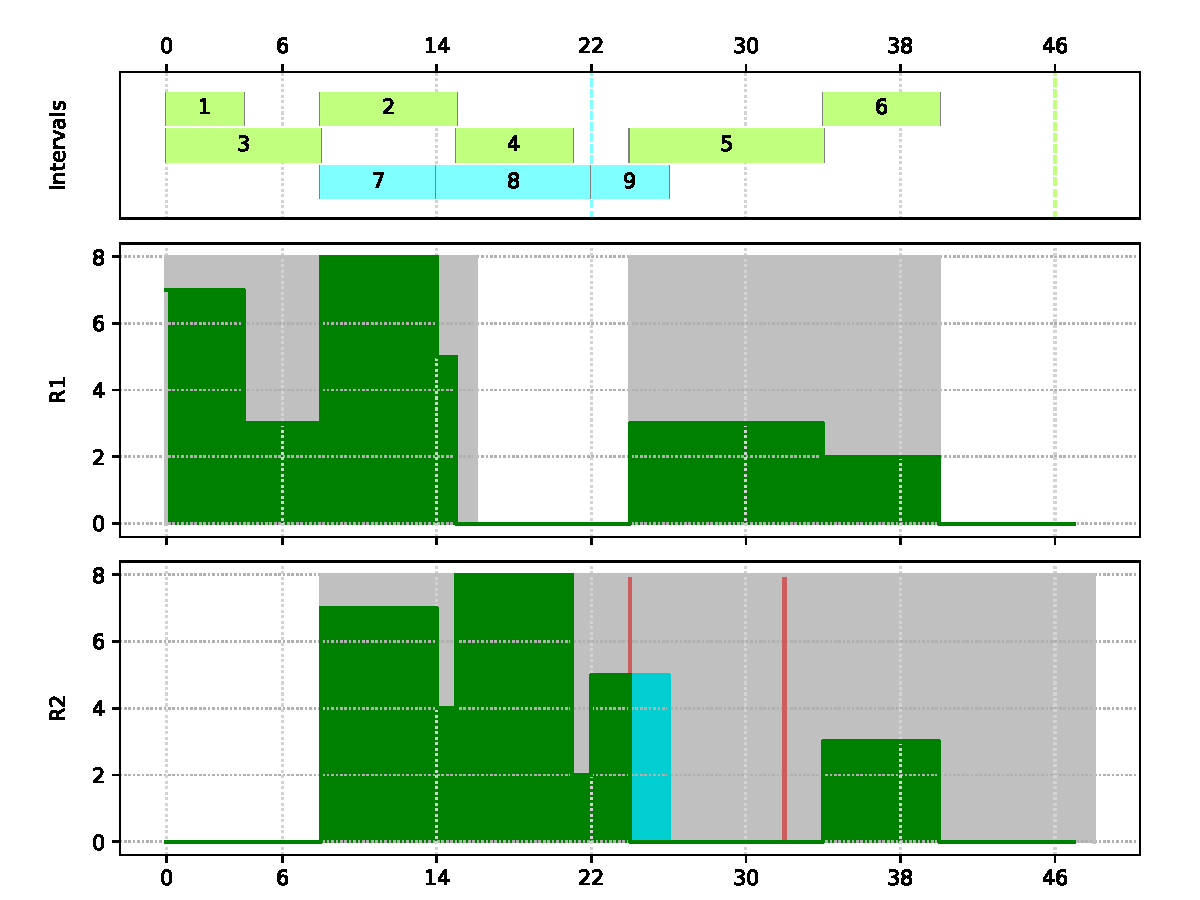
\includegraphics[width=0.85\textwidth]{img/example_solution_iira_intermediate.pdf}
    \caption{
        Computed example of an intermediate schedule obtained by the \ac{iira}
        ($\algIndicator = \indAUAU{}, \algGranularity = 8, \algConvolution = \convAround, \algMaxiter = 1, \algMaxperiods = 1, \algImprovement = 8$).
        The capacity of resource 2 is increased during the granular period
        spanning over time periods $\intinterval{24}{31}$.
        Subsequently, job 9 can be scheduled earlier.
        The newly introduced capacity utilized by the job 9 is highlighted.
    }
    \label{fig:example/iira-step}
\end{figure}

\begin{figure}[p]
    \centering
    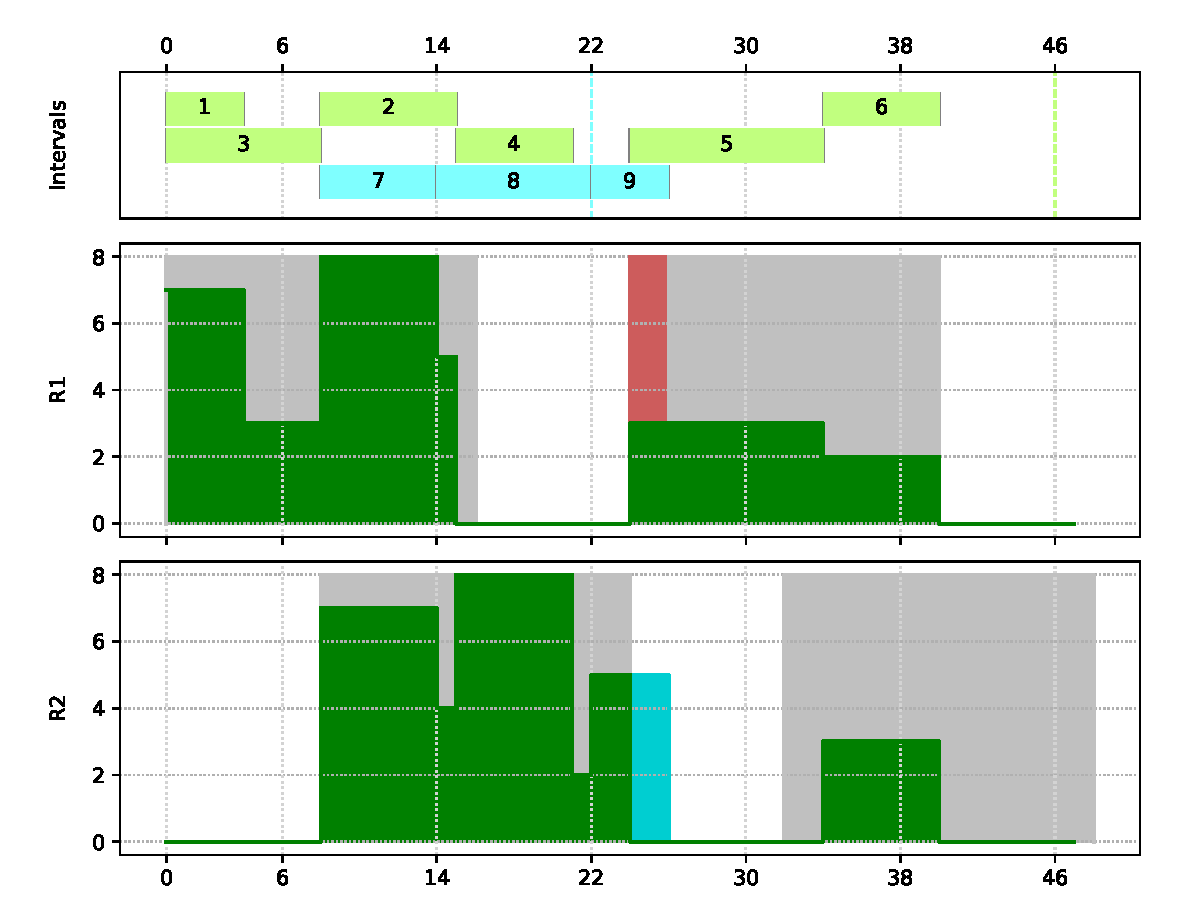
\includegraphics[width=0.85\textwidth]{img/example_solution_iira.pdf}
    \caption{
        Computed example of a schedule with reduced resource capacity functions obtained by the \ac{iira}
        ($\algIndicator = \indAUAU{}, \algGranularity = 8, \algConvolution = \convAround, \algMaxiter = 1, \algMaxperiods = 1, \algImprovement = 8$).
        The capacity of resource 2 is reduced during the granular period
        spanning over time periods $\intinterval{24}{31}$ to exclude unused capacity additions.
        The only additional capacity left is exactly the highlighted capacity consumed by the job 9.
    }
    \label{fig:example/iira-reduced}
\end{figure}

\begin{steps}
    \item
    First, the solution is evaluated using the given identification indicator
    and the bottleneck resource is identified by its maximal value of the identification indicator
    (lines~\ref{alg:iira/evaluation} and~\ref{alg:iira/identification}).

    \item
    The granular load of the bottleneck resource is computed
    and the improvement potentials for granular periods are computed
    using convolution (lines~\ref{alg:iira/granular-load} and~\ref{alg:iira/convolution}).
    The granular load of a resource indicates how is the resource being utilized during granular periods.
    High utilization could indicate a potential bottleneck.
    However, it is uncertain whether the bottleneck occurs in the highly-utilized granular period,
    or whether the high utilization is a consequence of a bottleneck
    in a preceding or a following granular period.
    This is why the granular load is convolved with a kernel function of choice,
    which propagates the information about high resource utilization
    to consecutive granular periods.
    The result of the convolution is trimmed to only contain "valid" values,
    i.e. values computed directly on the interval $\intinterval{1}{PC}$.
    \label{alg/iira-steps/identification}

    \item
    A small subset of granular periods is selected for the increase in capacity.
    The granular periods with the highest improvement potentials are chosen (line~\ref{alg:iira/periods}).
    The capacity of the bottleneck resource is increased during the selected granular periods
    by a specified amount (line~\ref{alg:iira/capacity-increase}).
    The modified resource capacity function of the bottleneck resources forms,
    together with the unchanged capacity functions of other resources,
    a new modified problem instance.
    Note that the algorithm does not consider the target order~$\targetOrder$ in any way
    when identifying bottlenecks (\cref{alg/iira-steps/identification})
    nor when selecting granular periods for capacity constraints relaxation.

    \item
    Finally, a new solution to the modified problem instance is found (line~\ref{alg:iira/modified-solution}).
    An example of a modified solution is given in \cref{fig:example/iira-step}.
    Based on this solution,
    reduced capacity functions are computed to exclude capacity relaxations
    not utilized in the solution (line~\ref{alg:iira/reduction}).
    An example of a schedule with reduced resource capacity functions is given in \cref{fig:example/iira-reduced}.
    The reduction involves the capacity functions of all the resources, not only of the bottleneck resource.
    This is because, in subsequent iterations of the algorithm,
    the introduction of new relaxations often leads to changes in the solution schedule.
    Such changes might cause previous relaxations to no longer be necessary,
    so in turn, every resource capacity function is reduced.
    Note that the function \algnameref{ReduceCapacityChanges}{alg:reduce-capacity-changes}
    takes the original resource capacity functions as input
    and the reductions are made with respect to them.
    As a final step, capacity migrations are computed in the reduced capacity functions
    to best utilize the existing unused capacities (line~\ref{alg:iira/additions-migrations}).
    Any remaining capacity requirements are then fulfilled with capacity additions.
\end{steps}

The algorithm utilizes multiple additional procedures and functions.
For brevity, we exclude the detailed specifics of the procedures
and instead offer short overviews of each procedure.
Complete pseudocodes of the procedures are available in \cref{sec:attachments/algorithms-functions-procedures}.

\begin{itemize}
    \item \algnameref{GranularResourceLoad}{alg:granular-resource-load}
        computes a granular resource load for a given resource.
        The granular load is a function mapping granular periods to the cumulative sum of the load
        of the resource over the specified granular period.
        Example of a computed granular load can is illustrated in \cref{fig:granular-load}.

        \begin{figure}[hbt]
            \centering
            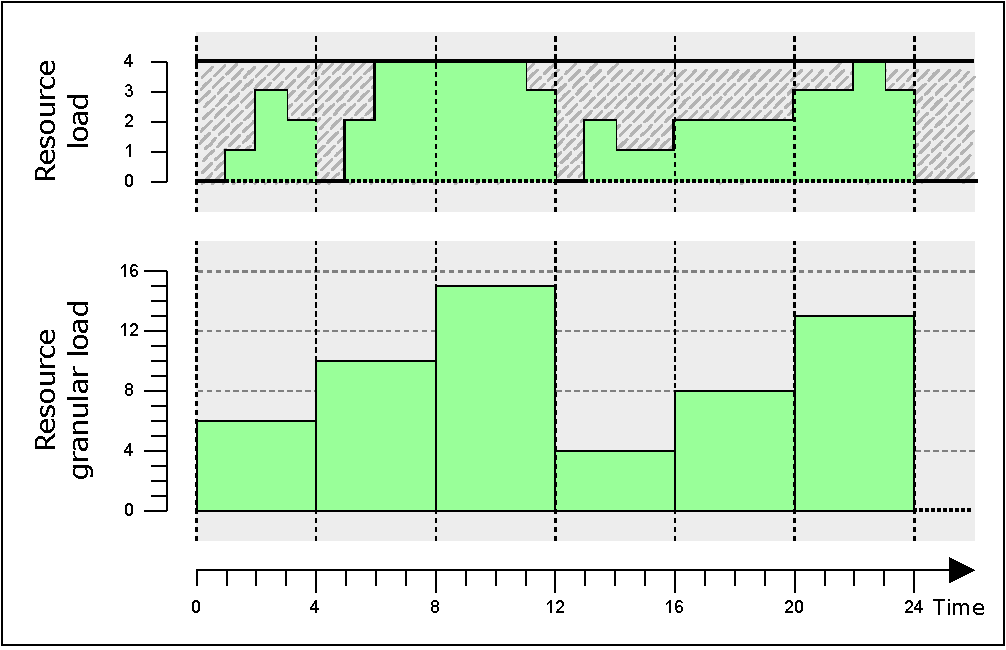
\includegraphics[width=0.85\textwidth]{img/GranularLoad.pdf}
            \caption{
                Resource granular load example.
                The first panel illustrates the resource load representing the consumption of jobs.
                The second panel illustrates the computed granular load with the granularity of 4 time periods.
                }
            \label{fig:granular-load}
        \end{figure}
        
    \item \algnameref{IncreaseGranularPeriodCapacity}{alg:increase-granular-period-capacity}
        increases the values of the given capacity function during the specified granular period.
        The capacity is increased in each time period covered by the granular period,
        determined by the specified granularity.

    \item \algnameref{ReduceCapacityChanges}{alg:reduce-capacity-changes}
        constructs reduced capacity functions for the given problem instance based on the original resource functions
        and the actual load of the instance resources (computed from the given solution).
        This function reduces redundant capacity additions introduced by former relaxations
        so that the resource capacity functions do not contain capacity additions not utilized by the solution.

    \item \algnameref{FindAdditionsAndMigrations}{alg:find-additions-and-migrations}
        finds capacity additions and migrations,
        as defined in \cref{subsec:problem-statement/bottlenecks/resource-capacity-modifications},
        for the resources of the given problem instance.
        In the same section,
        we discussed that in real-world production systems
        capacity migrations are preferred over capacity additions due to their comparatively small execution cost.
        Thus, we first find all possible migrations to utilize existing capacities.
        Then, when no other migrations are possible, the remaining capacity requirements are fulfilled
        by introducing capacity additions.
\end{itemize}

% ~~~~~~~~~~~~~~~~~~~~~~~~~~~~~~~~~~~~~~~~~~~~~~~~~~~~~~~~~~~~~~~~~~~~~~~~~~~~~~~~~~~~~~~~~~~~~~~~~~~~~~~~~~~
\section{Extended solution} \label{sec:solution-apporach/extended-solution}

In this section, we present a novel method for detecting bottlenecks
and relaxing related constraints in the \ac{rcpsp}.
The method is based on finding improvement intervals
in partially relaxed versions of the given problem.
A small subset of the improvement intervals is then selected and capacity constraints
corresponding to the selected improvement intervals are relaxed.
The primary goal is to identify relaxations that focus specifically on the target order.
By doing so, we hope to achieve great improvements in the tardiness of the target order
while maintaining low capacity modification costs and induced schedule differences.

% -----------------------------------------------------------------------------------------------------------
\subsection{Preliminaries} \label{subsec:solution-approach/extended-solutin/preliminaries}

Before we formulate the \acl{ssira},
we need to state a few definitions and ideas upon which the algorithm is designed.
First, we define the \emph{suffix-relaxed schedule} as a modification of an obtained schedule solution
where the algorithm finds improvement intervals.
We then define the \emph{left-shift closure} as a tool
for focusing the search for improvement intervals towards improving the tardiness of the target order.

\begin{defn}[Suffix-relaxed schedule] \label{def:suffix-relaxed-schedule}
    Let $\Schedule = (\jobstart{1}, \dots, \jobstart{n})$ be a schedule to a problem instance $\Instance$.
    Given a time period $t \in \intinterval{1}{\horizon}$,
    the \emph{suffix-relaxed schedule} for the time period $t$ is given by
    $\relaxedSchedule{t} = (\relaxedjobstart{t}{1}, \dots, \relaxedjobstart{t}{n})$, where
    $$
    \relaxedjobstart{t}{j} \defeq \begin{cases}
        \jobstart{j} & \text{if $\jobstart{j} \leq t$;} \\
        \max\left\{\relaxedjobstart{t}{i} + \duration{i}: \precedence{i}{j} \in \Precedences \right\} & \text{otherwise.}
    \end{cases}
    $$
\end{defn}

For a given job $j$, the value of $\relaxedjobstart{t}{j}$
depends only on the values $\relaxedjobstart{t}{i}$ of its precedence predecessors $i$,
given by precedences $\precedence{i}{j}$.
Since the precedence graph is directed and acyclic,
all values of $\relaxedSchedule{t}$ are well-defined and the definition is correct.

The suffix-relaxed schedule for a time period $t$ is a modification of the original schedule
where the start times of jobs starting in time periods up to $t$ remain unchanged,
and the start times of jobs scheduled to start later can be shifted to earlier time periods,
constrained only by precedence constraints.
This essentially relaxes resource capacity constraints for all jobs that, in the original schedule,
start after the time period $t$.

The idea is that a job scheduled during the later time periods could not be scheduled earlier
due to the lack of remaining capacity on the required resources,
assuming sufficient slack in precedence constraints.
By fully relaxing the resource capacity constraints in the suffix of a schedule,
we can compute potential starting times for jobs scheduled in that suffix,
had they not been constrained by the resource capacity constraints.
Following this, we can observe the potential improvements in the starting times
and the consequent required resource capacity relaxations.

\begin{defn}[Left-shift closure] \label{def:left-shift-closure}
    Let $\Schedule = (\jobstart{1}, \dots, \jobstart{n})$ be a schedule to a problem instance $\Instance$.
    A \emph{left-shift closure} of a job $j \in \Jobs$ is the set $\closure{j}~\subseteq~\Jobs$, where:
    \begin{conditions}
        \item
            $j \in \closure{j}$ \label{def:closure/base}

        \item
            All precedence predecessors directly preceding in the schedule are included.
            $$
            (\forall \precedence{i}{j} \in \Precedences):
            \jobend{i} = \jobstart{j} \implies \closure{i} \subset \closure{j}
            $$ \label{def:closure/precedence}
            \vspace{-2em}

        \item
            All jobs consuming a common resource directly preceding in the schedule are included.
            $$
            (\forall k \in \Resources, \consumption{j}{k} > 0)
            (\forall i \in \JobsOnResource{k}):
            \jobend{i} = \jobstart{j} \implies \closure{i} \subset \closure{j}
            $$ \label{def:closure/resource-precedence}
            \vspace{-2em}

        \item
            If $j$ is scheduled exactly at the start of a working shift,
            all jobs scheduled at the end of the previous working shift are included.
            \begin{multline*}
            (\forall k \in \Resources, \consumption{j}{k} > 0, \capacity{k}{\jobstart{j}-1} = 0)
            (\forall i \in \JobsOnResource{k}):
            \\
            \mathrm{ps}_k(\jobstart{j}) - \duration{j} \leq \jobend{i} \leq \mathrm{ps}_k(\jobstart{j})
            \implies \closure{i} \subset \closure{j}
            \end{multline*} \label{def:closure/shift-pause-precedence}
            where $\mathrm{ps}_k(t) \defeq \max\{t^\prime \in \intinterval{1}{t-1} : \capacity{k}{t^\prime} > 0\}$.
    \end{conditions}
\end{defn}

The left-shift closure of a job $j$ defines the set of all jobs
preventing the job $j$ from starting in an earlier time period.
The only exception to this interpretation is the \cref{def:closure/base},
which simplifies the inductive definition.

\Cref{def:closure/precedence} states that a direct predecessor $i$ of the job $j$,
indicated by the precedence constraint $\precedence{i}{j}$,
is included in $\closure{j}$ if the jobs are scheduled consecutively.
Jobs $i$ and $j$ are scheduled consecutively if the execution of the job~$i$ ends
at the exact same time period where the execution of the job $j$ starts,
i.e. $\jobend{i} = \jobstart{j}$.

\Cref{def:closure/resource-precedence} involves all jobs scheduled consecutively with the job $j$,
which share at least one required resource.
Jobs can be executed on multiple resources,
but sharing just one resource is sufficient for the jobs to influence each other.
This resource requirement overlap can delay the job $j$ if its predecessor job $i$'s resource consumption
prevents the job $j$ from being scheduled earlier.

Lastly, \cref{def:closure/shift-pause-precedence} involves jobs at the end of previous working shifts.
Assuming sufficient slack in precedence constraints,
the job $j$ starts exactly at the start of a working shift because
it could not have been scheduled at the end of the previous working shift
due to the lack of remaining capacities on its required resources.
Jobs scheduled at the end of the previous working shift consume the required resources
and thus prevent the job $j$ from being scheduled there.

\begin{figure}[p]
    \centering
    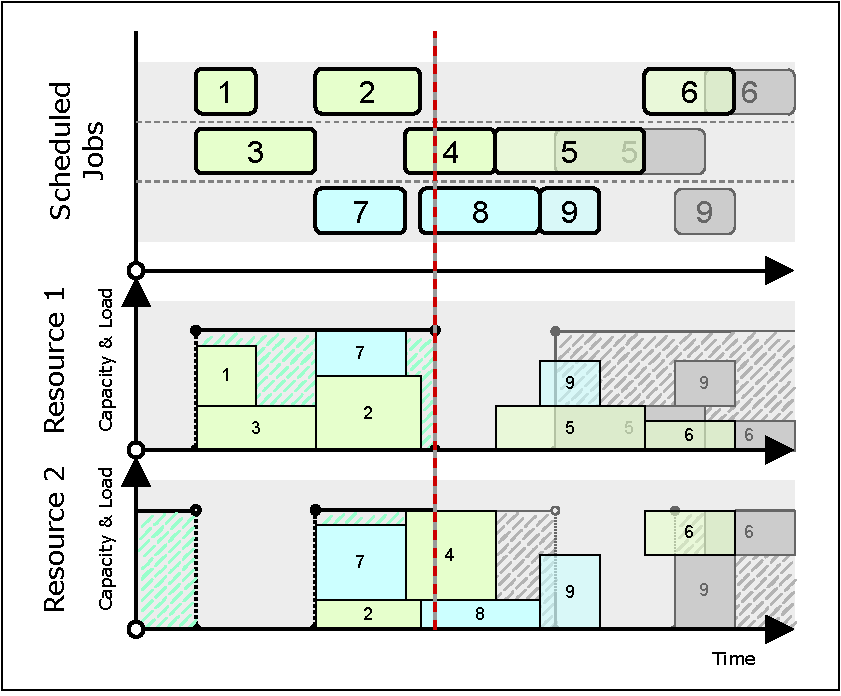
\includegraphics[width=0.7\textwidth]{img/Schedule-Relaxed.pdf}
    \caption{
        Example of a suffix-relaxed schedule based on the schedule given in \cref{fig:schedule}.
        The red vertical line represents the time period for which the suffix-relaxed schedule was computed.
        The resource capacity constraints were relaxed for jobs 5, 6, and 9
        as they were scheduled later than the specified time period.
        We observe that in the relaxed schedule,
        job 9 would require only small capacity additions on both resources,
        should it be scheduled on them.
        Moreover, most of the requirements could be satisfied
        by migrating unused capacities between the resources.
        }
    \label{fig:schedule-relaxed}
\end{figure}

\begin{figure}[p]
    \centering
    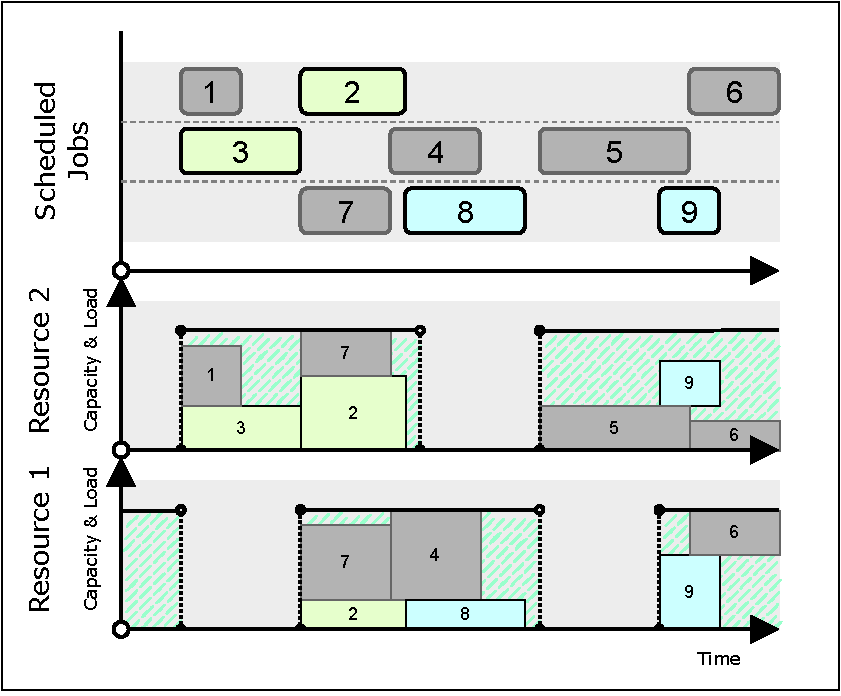
\includegraphics[width=0.7\textwidth]{img/Schedule-Closure.pdf}
    \caption{
        Example of a left-shift closure computed for the job 9 in the schedule given in \cref{fig:schedule}.
        Here, the left-shift closure of the job 9 is the set $\closure{9} = \{ 2, 8, 9 \}$.
        The included jobs are highlighted; jobs not included are dimmed.
        Job 9 is trivially included by \cref{def:closure/base}.
        Job 8 is included by \cref{def:closure/shift-pause-precedence} --- pauses in resource working shifts.
        Job 2 is included by \cref{def:closure/resource-precedence} --- resource predecessor of the job 8 on resource 2.
        Conversely, job 3 ends at the same time period job 2 starts, however, they are not precedence predecessors
        and thus job 3 is not included.
        }
    \label{fig:schedule-closure}
\end{figure}

% -----------------------------------------------------------------------------------------------------------
\subsection{Schedule Suffix Interval Relaxing Algorithm} \label{subsec:extended-solution/schedule-suffix-interal-relaxing-algorithm}

Having presented the main concepts in the previous section,
we now formulate the \acf{ssira} in \cref{alg:schedule-suffix-interval-relaxing-algorithm}.
The formulation of the algorithm itself is quite simple.
The core procedure is encapsulated in the
\algnameref{Find\-Intervals\-To\-Relax}{alg:find-intervals-to-relax} function,
formulated in \cref{alg:find-intervals-to-relax}.


\begin{algorithm}[t]
\caption{\acf{ssira}}
\label{alg:schedule-suffix-interval-relaxing-algorithm}
\begin{algorithmic}[1]

\Params  Iterations limit $\algMaxiter$, improvement intervals limit $\algMaxintervals$,
\Paramsc interval sort key $\algSortkey$
\Input  Solution $\Schedule$ to a problem instance $\Instance$, target order $\targetOrder$

\State $\Instance^* \gets \Instance$, $\Schedule^* \gets \Schedule$
       \Comment Modified instance and its solution, initially
       \Statecr copies of the original instance and solution
\Repeat \label{alg:ssira/repeat}
    \State $\chi_1, \dots, \chi_{\algMaxintervals} \gets$ \Callref{FindIntervalsToRelax}%
                                                                  {$\Instance^*$, $\Schedule^*$, $\algMaxintervals$, $\algSortkey$, $\targetOrder$}%
                                                                  {alg:find-intervals-to-relax}
                                                                  \label{alg:ssira/ints}
    \State $\capacityf{1}^*, \dots, \capacityf{m}^* \gets$ \Callref{ModifyResourceCapacities}%
                                                                   {$\Instance^*$, $\chi_1, \dots, \chi_{\algMaxintervals}$}%
                                                                   {alg:modify-resource-capacities}
                                                                   \label{alg:ssira/modify}
    \State Find solution $\Schedule^*$ to the modified instance $\Instance^*$ \label{alg:ssira/solution}
    \State $\capacityf{1}^*, \dots, \capacityf{m}^* \gets$ \Callref{ReduceCapacityChanges}%
                                                                   {$\Instance^*$, $\Schedule^*$, $\capacityf{1},$ \dots, $\capacityf{m}$}%
                                                                   {alg:reduce-capacity-changes}
                                                                   \label{alg:ssira/reduction}
    \State $\Additions^{\Instance^*}, \Migrations^{\Instance^*} \gets $
           \Callref{FindAdditionsAndMigrations}%
                   {$\Instance^*$, $\Schedule^*$}%
                   {alg:find-additions-and-migrations}
                   \label{alg:ssira/additions-migrations}
\ForIter{$\algMaxiter$} \label{alg:ssira/for-iters}

\Output  Modified instance $\Instance^*$ and its solution $\Schedule^*$,
\Outputc additions $\Additions^{\Instance^*}$, migrations $\Migrations^{\Instance^*}$
\end{algorithmic}
\end{algorithm}


\begin{algorithm}[t]
\caption{FindIntervalsToRelax}
\label{alg:find-intervals-to-relax}
\begin{algorithmic}[1]

\Input  Problem instance $\Instance$, its solution $\Schedule$, improvement intervals limit $\algMaxintervals$,
\Inputc interval sort key $\algSortkey$, target order $\targetOrder$

\For {$t \in \intinterval{1}{\horizon}$}
    $\relaxedSchedule{t} \gets$ \Callref{ComputeSuffixRelaxedSchedule}%
                                        {$\Instance$, $\Schedule$, $t$}%
                                        {alg:suffix-relaxed-schedule}  \label{alg:ssira/ints/schedule-suffixes}
\EndFor
\State $\closure{\targetOrder} \gets$ \Callref{ComputeLeftShiftClosure}%
                                              {$\Instance$, $\Schedule$, $\targetOrder$}%
                                              {alg:left-shift-closure}  \label{alg:ssira/ints/closure}
\State $X \gets \emptyset$  \label{alg:ssira/ints/ints-init}
\For {$j \in \closure{\targetOrder}$}
    \State $s \gets \min_t \left\{ \relaxedjobstart{t}{j} : \relaxedjobstart{t}{j} < \jobstart{j} \right\}$  \label{alg:ssira/ints/ints-improvement}
        \Comment Find the earliest improvement
    \State $X \gets X \cup \left\{ (j,\; s,\; s + \duration{j}) \right\}$  \label{alg:ssira/ints/ints-inclusion}
\EndFor

\State $\chi_1, \dots, \chi_{\algMaxintervals} \gets$ first $\algMaxintervals$ intervals from $X$ ordered by $\algSortkey$  \label{alg:ssira/ints/select-imp-ints}

\Output  Improvement intervals $\chi_1, \dots, \chi_{\algMaxintervals}$,
\Outputc a set of 3-tuples $(j, s, e) \in \Jobs \times \intinterval{1}{\horizon}^2$
\end{algorithmic}
\end{algorithm}

\begin{figure}[p]
    \centering
    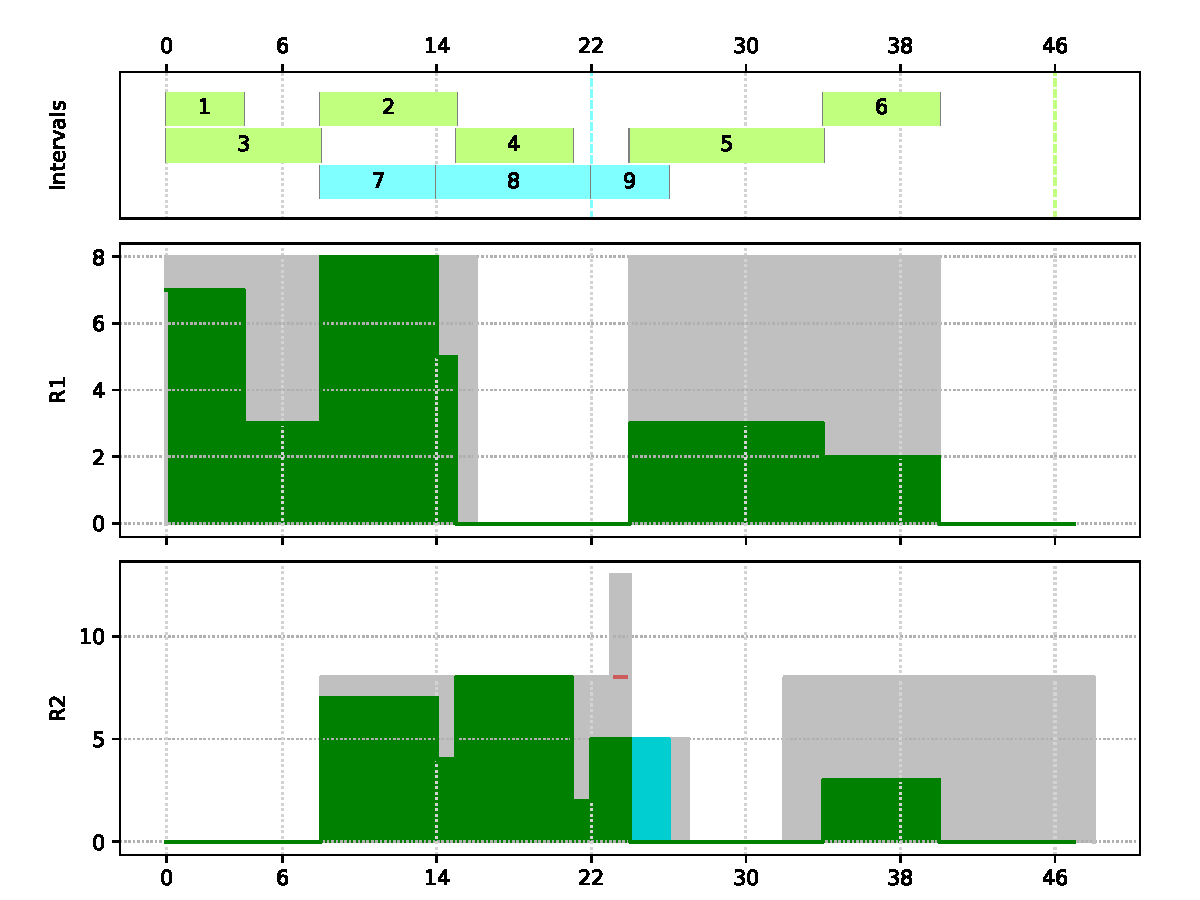
\includegraphics[width=0.85\textwidth]{img/example_solution_ssira_intermediate.pdf}
    \caption{
        Computed example of an intermediate schedule obtained by the \ac{ssira}
        ($\algMaxiter = 1, \algMaxintervals = 1, \algSortkey = \algSortkeyTime$).
        The capacity of resource 2 is increased over the improvement interval
        spanning the time periods $\intinterval{22}{27}$.
        Subsequently, job 9 can be scheduled earlier.
        The newly introduced capacity utilized by the job 9 is highlighted.
        Note that the job 9 is scheduled earlier than anticipated by the improvement interval.
    }
    \label{fig:example/ssira-step}
\end{figure}

\begin{figure}[p]
    \centering
    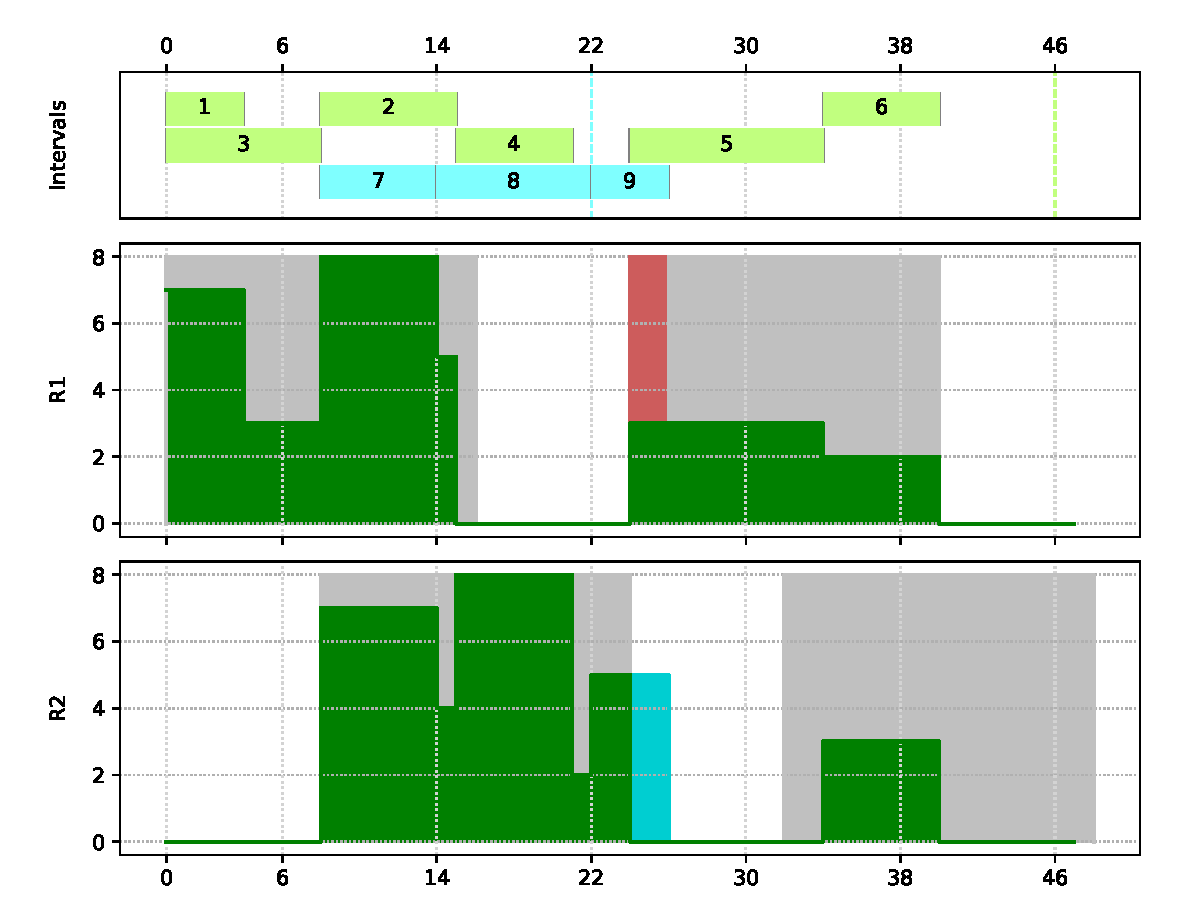
\includegraphics[width=0.85\textwidth]{img/example_solution_ssira.pdf}
    \caption{
        Computed example of a schedule with reduced resource capacity functions obtained by the \ac{ssira}
        ($\algMaxiter = 1, \algMaxintervals = 1, \algSortkey = \algSortkeyTime$).
        The capacity of resource 2 is reduced,
        removing unused capacities introduced in \cref{fig:example/ssira-step}.
        The only additional capacity left is the highlighted capacity consumed by the job 9 migrated from resource 1.
        Note that this schedule is identical to the schedule obtained by the \ac{iira} in \cref{fig:example/iira-reduced}.
    }
    \label{fig:example/ssira-reduced}
\end{figure}

The \ac{ssira} consists of a main loop (lines~\ref{alg:ssira/repeat}--\ref{alg:ssira/for-iters}),
the input of which is a problem instance and its solution,
the output of which is a modified problem instance and its solution.
In each iteration of the main loop, the algorithm first finds improvement intervals (line~\ref{alg:ssira/ints}).
Then, resource capacity functions are modified based on these intervals (line~\ref{alg:ssira/modify}).
The subsequent steps (lines~\ref{alg:ssira/solution}--\ref{alg:ssira/additions-migrations}) mirror those of the \ac{iira},
as stated in detail in \cref{subsec:solution-approach/baseline-solution/iira}.
A new solution to the modified problem instance is found,
the modified resource capacity functions are reduced based on that solution,
and capacity migrations and additions are computed in the reduced capacity functions.
An example of a schedule obtained in the modified instance is given in \cref{fig:example/ssira-step}
and that schedule with reduced capacity functions is given in \cref{fig:example/ssira-reduced}.
Note that in this example, both the \ac{iira} and the \ac{ssira} obtained the same solution,
given in \cref{fig:example/iira-reduced} and \cref{fig:example/ssira-reduced} respectively.

The \algnameref{FindIntervalsToRelax}{alg:find-intervals-to-relax} function consists of initializations,
the search for improvement intervals, and a preference-selection of intervals.
We describe the individual steps performed in the function in the following outline.

\begin{steps}
    \item
        Suffix-relaxed schedules are computed for each time period within the scheduling horizon
        (line~\ref{alg:ssira/ints/schedule-suffixes}).
        These schedules represent all possible job-interval relaxations,
        from which potential improvement intervals are subsequently identified and selected.
        Following this, the left-shift closure of the target order is computed (line~\ref{alg:ssira/ints/closure}).
        This closure represents the set of jobs considered for improvement.

    \item
        Potential improvement intervals are identified iteratively
        for jobs within the left-shift closure of the target order
        (lines~\ref{alg:ssira/ints/ints-init}--\ref{alg:ssira/ints/ints-inclusion}).
        For each job in the closure,
        the start of the potential improvement interval is determined
        as the earliest improving time for that job across all suffix-relaxed schedules
        (line~\ref{alg:ssira/ints/ints-improvement}).
        The start time of a job in a suffix-relaxed schedule is considered improving
        if it is earlier than the start time in the original schedule.
        Then, the potential improvement interval for the job is constructed (line~\ref{alg:ssira/ints/ints-inclusion}),
        incorporating the identified earliest improving time and the job's execution duration.
        The constructed potential improvement interval is added to the set of potential improvement intervals
        for the subsequent selection of preferred improvement intervals.

    \item
        Predefined number of improvement intervals is selected based on a specified sort key
        (line~\ref{alg:ssira/ints/select-imp-ints}).
        The potential improvement intervals are ordered according to the sort key,
        and the first intervals from this ordering are selected as the proposed improvement intervals.
\end{steps}

The \ac{ssira} and the \algnameref{FindIntervalsToRelax}{alg:find-intervals-to-relax} function
both utilize multiple additional procedures and functions.
The \algnameref{ReduceCapacityChanges}{alg:reduce-capacity-changes}
and \algnameref{FindAdditionsAndMigrations}{alg:find-additions-and-migrations}
functions used by the \ac{ssira} are the same functions as those used by the \ac{iira}.
Their overview was given in \cref{subsec:solution-approach/baseline-solution/iira}.
For brevity, we exclude the detailed specifics of the
remaining functions and instead offer their short overviews.
Complete pseudocodes of the functions are available in \cref{sec:attachments/algorithms-functions-procedures}.

\begin{itemize}
    \item \algnameref{ModifyResourceCapacities}{alg:modify-resource-capacities}
        modifies the resource capacity functions of a given problem instance
        by increasing their capacities within the specified improvement intervals.
        Each improvement interval is associated with a particular job.
        For every resource required by that job,
        its resource capacity function is increased by the job's required resource consumption of that resource
        over the duration of the improvement interval.

    \item \algnameref{ComputeSuffixRelaxedSchedule}{alg:suffix-relaxed-schedule}
        computes the suffix-relaxed schedule for a specified time period,
        as defined in \cref{def:suffix-relaxed-schedule}.
        Initially, the topological order of the jobs in the instance is computed.
        Then, for each job considered in the topological order,
        its start time in the suffix-relaxed schedule is determined:
        if the job was scheduled up to the specified time period,
        its original start time is used;
        otherwise, the latest end time of its precedence predecessors is computed in the suffix-relaxed schedule,
        and this value is used.
        This maximum is well-defined due to the jobs being processed in topological ordering and thus,
        all values have been determined by the time they are first considered in the maxima.

    \item \algnameref{ComputeLeftShiftClosure}{alg:left-shift-closure}
        computes the left-shift closure of a specified job, as defined in \cref{def:left-shift-closure}.
        The precedence graph is traversed in a breadth-first manner, starting from the specified job.
        The traversal considers only the jobs that correspond to the defining
        \cref{def:closure/precedence,def:closure/resource-precedence,def:closure/shift-pause-precedence}.
\end{itemize}

\chapter{Numerical experiments}

\chapwithtoc{Conclusion} \label{chap:conclussion}

\todo{Contribution}

\todo{Result summary}

\todo{Further research directions}
\begin{itemize}
    \item
        Sensitivity analysis was not conducted.
        Following the work of \citet{Lawrence1994},
        the effect of our proposed changes could be studied
        to evaluate how the changes affect the sensitivity of the system.
\end{itemize}


%%% Bibliography
%%% Bibliography (literature used as a source)
%%%
%%% We employ biblatex to construct the bibliography. It processes
%%% citations in the text (e.g., the \cite{...} macro) and looks up
%%% relevant entries in the bibliography.bib file.
%%%
%%% See also biblatex settings in thesis.tex.

%%% Generate the bibliography. Beware that if you cited no works,
%%% the empty list will be omitted completely.

% We let bibliography items stick out of the right margin a little
\def\bibfont{\hfuzz=2pt}

\printbibliography[heading=bibintoc]

%%% If case you prefer to write the bibliography manually (without biblatex),
%%% you can use the following. Please follow the ISO 690 standard and
%%% citation conventions of your field of research.

% \begin{thebibliography}{99}
%
% \bibitem{lamport94}
%   {\sc Lamport,} Leslie.
%   \emph{\LaTeX: A Document Preparation System}.
%   2nd edition.
%   Massachusetts: Addison Wesley, 1994.
%   ISBN 0-201-52983-1.
%
% \end{thebibliography}


%%% Figures used in the thesis (consider if this is needed)
% \listoffigures

%%% Tables used in the thesis (consider if this is needed)
%%% In mathematical theses, it could be better to move the list of tables to the beginning of the thesis.
% \listoftables

%%% Abbreviations used in the thesis, if any, including their explanation
%%% In mathematical theses, it could be better to move the list of abbreviations to the beginning of the thesis.
\chapwithtoc{Notation} \label{sec:notation}

\todo{Additional entries}
\begin{table}[h!]
    \centering
    \begin{tabularx}{\textwidth}{lX}
        \textbf{Symbol} & \textbf{Definition} \\
        \hline
        \\

        \textbf{Problem instances}      & \cellrule \\
        $\Instance = (\Jobs, \Precedences, \Resources, \Orders, \horizon)$ & Problem instance \\
        $\Jobs = \{ 1, \dots, n \}$     & Set of jobs \\
        $\duration{j}$                  & Processing time of job~$j$ \\
        $\deadline{j}$                  & Deadline for a job~$j$ \\
        $\tardinessweight{j}$           & Tardiness weight for a job~$j$ \\
        $\precedence{i}{j}$ or $(i,j)$  & Precedence between jobs $i$ and $j$ \\
        $\Precedences$                  & Set of precedences \\
        $G = (\Jobs, \Precedences)$     & Precedence graph \\
        $\Resources = \{1, \dots, m\}$  & Set of resources \\
        $\capacityf{k}$                 & Capacity function of resource~$k$ \\
        $\capacity{k}{t}$               & Capacity of resource $k$ in time period~$t$ \\
        $\shiftcapacity{k}$             & Shift capacity of a resource~$k$ \\
        $\consumption{j}{k}$            & Per-period consumption of a resource~$k$ by a~job~$j$ \\
        $\horizon$                      & Time horizon \\
        $1, \dots, \horizon$            & Time periods \\
        $\JobsOnResource{k}$
            & The set of jobs executed on the resource~$k$ \\
        $\JobsOnResourceInTimePeriod{k}{t}$
            & The set of jobs executed on the resource~$k$ during the time period~$t$ \\
        $\JobsOnResourceInPeriod{k}{i}$
            & The set of jobs executed on the resource~$k$ during the uninterrupted active period~$i$\\
        \\

        \textbf{Schedules, solutions}   & \cellrule \\
        $\jobstart{j}$                                      & Start time of job~$j$ \\
        $\Schedule = (\jobstart{1}, \dots, \jobstart{n})$   & Schedule \\
        $\jobend{j} = \jobstart{j} + \duration{j}$          & Completion time of job~$j$ \\
        $\Completions = (\jobend{1}, \dots, \jobend{n})$    & All completion times of jobs \\
        \\

        \textbf{Identification indicators} & \cellrule \\
        
        $\indMUR{k}$                                                    & \acl{mur} \\
        $\indAUAD{k}$                                                   & \acl{auad} \\
        $\indRS{k},\; \indRC{k}$                                        & \acl{rs}, \acl{rc} \\
        $\indMRUR{k}$                                                   & \acl{mrur} \\
        $\indAUAU{k}$                                                   & \acl{auau} \\
        $\indPRU{k}{i}$                                                 & \acl{pru} \\
        \\

        \tablenote{2}{supper-scripting a value with a schedule symbol --- for example
        $\jobend{j}^{\Schedule}$ --- relates that value to the specified schedule.} \\
    \end{tabularx}
\end{table}



%%% Doctoral theses must contain a list of author's publications
\ifx\ThesisType\TypePhD
\chapwithtoc{List of Publications}
\fi

%%% Attachments to the thesis, if any. Each attachment must be referred to
%%% at least once from the text of the thesis. Attachments are numbered.
%%%
%%% The printed version should preferably contain attachments, which can be
%%% read (additional tables and charts, supplementary text, examples of
%%% program output, etc.). The electronic version is more suited for attachments
%%% which will likely be used in an electronic form rather than read (program
%%% source code, data files, interactive charts, etc.). Electronic attachments
%%% should be uploaded to SIS. Allowed file formats are specified in provision
%%% of the rector no. 72/2017. Exceptions can be approved by faculty's coordinator.
\appendix
\chapter{Attachments} \label{chap:attachments}

% ~~~~~~~~~~~~~~~~~~~~~~~~~~~~~~~~~~~~~~~~~~~~~~~~~~~~~~~~~~~~~~~~~~~~~~~~~~~~~~~~~~~~~~~~~~~~~~~~~~~~~~~~~~~
\section{Algorithms, Functions, and Procedures} \label{sec:attachments/algorithms-functions-procedures}


\begin{alg}{Function}{GranularResourceLoad}{$k$, $\Instance$, $\Schedule$, $PC$} \label{alg:granular-resource-load}
\State $L : \intinterval{1}{PC} \to \Nzero$
       \Comment Period load function
\For {$j \in \JobsOnResource{k}$}
    \State $i_l \gets \lfloor \jobstart{j} / \algGranularity \rfloor$,
           \Comment{First overlapping period}
    \State $i_h \gets \lfloor \jobend{j} / \algGranularity \rfloor$
           \Comment{Last overlapping period}
    \If {$i_l = i_h$}
        \Comment{If the job overlaps with a single period...}
        \State $L(i_l) \gets L(i_l) + \duration{j} \consumption{j}{k}$
    \Else
        \Comment{...the job overlaps with multiple periods}
        \State $L(i_l) \gets L(i_l) + (\algGranularity (i_l + 1) - \jobstart{j}) \cdot \consumption{j}{k}$
        \For {$i \in \intinterval{i_l+1}{i_h-1}$}
            \State $L(i) \gets L(i) + \algGranularity \cdot \consumption{j}{k}$
        \EndFor
        \State $L(i_h) \gets L(i_h) + (\jobend{j} - \algGranularity (i_h - 1)) \cdot c$
    \EndIf
\EndFor
\State \Return $L$
\end{alg}


\begin{alg}{Function}{IncreaseGranularPeriodCapacity}{$i$, $\capacityf{k}$, $\algGranularity$, $\algImprovement$} \label{alg:increase-granular-period-capacity}
\State $t_l \gets 1+ (i-1)\algGranularity$
       \Comment First time period covered
\State $t_h \gets i \algGranularity$
       \Comment Last time period covered
\For{$t \in \intinterval{t_l}{t_h}$}
    \State $\capacity{k}{t} \gets \capacity{k}{t} + \algImprovement$
\EndFor
\State \Return $\capacity{k}{t}$
\end{alg}


\begin{alg}{Function}{ReduceCapacityChanges}{$k$, $\capacityf{\text{orig}}$, $\Instance$, $\Schedule$} \label{alg:reduce-capacity-changes}
\State $\capacityf{}^\prime: \intinterval{1}{\horizon} \to \Nzero$
       \Comment Reduced capacity function
\State $L \gets $ \Call{ResourceLoad}{$k$, $\Instance$, $\Schedule$}
\For {$t \in \intinterval{1}{\horizon}$}
    \State $\capacity{}{t}^\prime \gets \max(\capacity{\text{orig}}{t}, L(t))$
\EndFor
\State \Return $\capacityf{}^\prime$
\end{alg}


\begin{alg}{Function}{ResourceLoad}{$k$, $\Instance$, $\Schedule$} \label{alg:resource-load}
\State $L : \intinterval{1}{\horizon} \to \Nzero$
\For {$t \in \intinterval{1}{\horizon}$}
    \State $L(t) \gets \sum_{j \in \JobsOnResourceInTimePeriod{k}{t}} \consumption{j}{k}$
        \Comment $\JobsOnResourceInTimePeriod{k}{t}$ with respect to given schedule $\Schedule$
\EndFor
\State \Return $L$
\end{alg}


\begin{alg}{Function}{FindAdditionsAndMigrations}{...} \label{alg:find-additions-and-migrations}
\State TODo
\end{alg}




\end{document}
